%!TEX root =../MacbethThesis.tex
\acresetall
\chapter{Simulation of a Knowledge Commons}\label{ch:results}

\lettrine[lines=3]{I}{n} this chapter we present a computer model of participatory sensing and use
this model to test our theory that by managing information and knowledge as a
commons, and according to Ostrom's principles for sustainable management of
common-pool resources we can improve the outcomes for agents in this system.

We first describe our model of participatory sensing, which approximates a
participatory sensing campaign as a reinforcement learning problem. This
approximation allows us to abstract the details of individual campaigns and
simply reason about where utility is accrued in the system.  We describe the
implementation of our simulation model, which combines an abstract
reinforcement learning problem with the provision and appropriation system
outlined in \autoref{sec:iad}. This model is implemented using Presage2, with
institutional rules processed by Drools-EInst. We then describe the results of
a series of experiments with this simulation model.

\section{Modelling Participatory Sensing as a Reinforcement Learning Problem}

So far we have articulated participatory sensing as the contribution of
information by individuals to a pool. This collected information can then be
used to generate new derived information using some kind of knowledge.
However, we have yet to describe what this knowledge is.

In general, an algorithm which takes data as an input and gives information
about the data as an output can be classified as a \emph{machine learning}
algorithm. Data aggregation in participatory-sensing applications follows this
pattern. There are three main types of machine learning. \emph{Supervised
learning} takes data which has been labelled by an expert, and aims to learn
how to predict this label for unlabelled data; \emph{unsupervised learning}
looks for patterns in unlabelled data; and in \emph{reinforcement learning}
performs actions and receives feedback from an environment, and aims to chose
actions which receive the highest rewards.

Participatory sensing may deal with either of these types of machine learning.
Using raw sensor readings of, for example, temperature, and using them to
predict future temperatures would be \emph{unsupervised} learning from sensing
data. If these readings also had a user specified `comfort' level attached to
them, then we could use \emph{supervised} learning to work out if comfort
level is correlated with temperature and infer expected comfort levels from
temperature data. \emph{Reinforcement learning} would be used when the output
of the sensing process informs actions to be taking in the same environment
that sensing is done.

When viewing participatory sensing as an agent-based system, we can see that
information is often generated as a result of an action: that of taking a sensor
reading. This information, when combined with other information and processed
by a suitable machine learning algorithm, leads to derived information with
some additional value. In most cases, part of this value is offered back to
the original gatherer as an incentive to contribute. In many cases this
information improves a decision process in the agent, and the whole sensing
process can be seen as an optimisation feedback loop. Consider some of our
reviewed examples from \autoref{ch:kc}:

\begin{itemize}
\item Pothole Patrol~\citep{Eriksson2008}, VTrack~\citep{Thiagarajan2009}, Parknet~\citep{Mathur2010} and Waze all use information from participating cars to provide optimised route information back to them, such that they can reach their destination quicker, avoid hazards and so on.
\item With LiveCompare~\citep{Deng2009} users can derive reduced grocery costs from the information provided via the app.
\item Cloud2Bubble~\citep{Costa2012} gives feedback to users to improve their comfort levels during public transportation journeys.
\end{itemize}

These can be seen as reinforcement learning problems. Users are taking
repeated actions, such as driving, buying grocery items or taking public
transportation, and each time deriving both utility and information from the
process. This can be then used to optimise the process for the next iteration.
This process can be done individually, but participatory sensing can
significantly speed up this learning process.

Reinforcement learning is a form of machine learning where one aims to
determine which sequence of actions to take in order to maximise a cumulative
reward. This is a method of learning while interacting with the environment,
and based on the feedback given from each action. It differs from supervised
learning in that the agent is not provided with examples, it must learn
through trying actions. This reveals an important trade-off in reinforcement
learning, that of \emph{exploitation} vs. \emph{exploration}. This trade-off
is between exploiting a known good strategy and exploring unknown strategies
for one which may be better~\citep{Sutton1998}.

Participatory sensing is particularly useful for these kinds of problems as it
can reduce the need for exploration. In the case of vehicle navigation an
individual would have to do significant exploration to find a suitable route
in a new area. Expanding the number of vehicles contributing data allows
individuals to navigate new areas with little exploration required, and
therefore derive a better utility.

In most practical participatory-sensing applications, the aim is to infer the
utility of actions from the provided information and then provide advice on
the best action to perform next. For our model we simplify this process by
making the information provided be the actual utility observed. This allows us
to frame a participatory sensing problem within the abstract reinforcement
learning framework, defined by \citet{Sutton1998}.

This framework, defines an \emph{agent} which interacts with an
\emph{environment} in discrete time-steps. Each time-step the agent receives
the environment's state and selects an action from the set of those available
from the current state. Then in the next time-step the agent receives a reward
from his action, and the new state and the process continues. The decision
about which action to take is done by the agent's \emph{policy}, and this is
what reinforcement learning aims to improve. The agent's goal is to maximise its
total accrued reward.

We instantiate this framework with multiple agents in a shared environment.
Within this environment there are institutions available which provide
\emph{policies} via \emph{provision} and \emph{appropriation} actions.  The
integration of reinforcement learning with a provision and appropriation
system is shown in \autoref{fig:reinflearn}. When in a state at time $t$,
$s_t$, an agent performs an action $a_t$, resulting in a new state $s_{t+1}$,
and a reward $r_{t+1}$. Unlike in a standard reinforcement learning scenario,
where the agent's own learning \emph{policy} is used, the agent provisions a
tuple  $(a_t,s_t,s_{t+1},r_{t+1})$ (describing this observation of environment
behaviour), and then appropriates a suggested next action $a_{t+1}$, from an
institution.

\begin{figure}
\centering
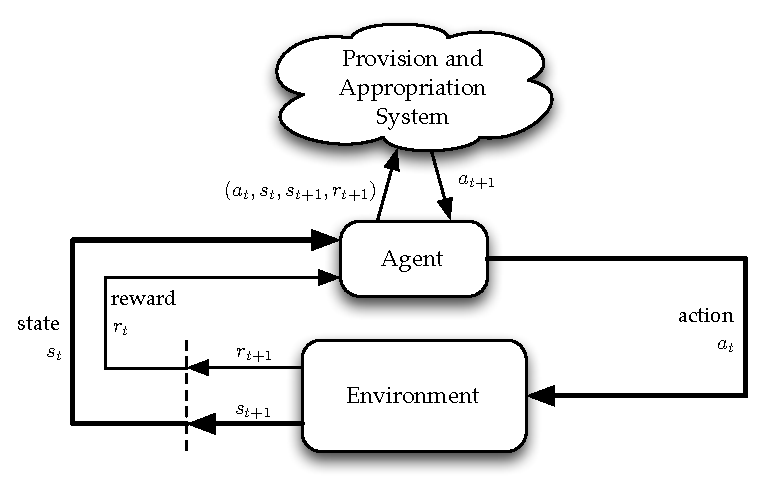
\includegraphics{gfx/reinforcementlearning}
\caption[Abstract reinforcement framework integrated with a provision and appropriation system]{Abstract reinforcement framework integrated with a provision and appropriation system (adapted from \citet[p.52]{Sutton1998}).}\label{fig:reinflearn}
\end{figure}

This model integrates the reinforcement learning framework with our framework
for participatory sensing as a provision and appropriation system from
\autoref{sec:iad}. The provision and appropriation actions from reinforcement
learning agents match those of \emph{gatherers} and \emph{consumers}.
\emph{Policies} are provided by \emph{analysts}. In our model we do not use
\emph{evaluators}, however they could be added to provide meta level analysis
of the quality of \emph{policies}, by determining the efficacy of actions
suggested by them.

% TODO: figure, prov and app system linked to game

% There are several issues when considering how to model a generic machine learning problem:
% \begin{itemize}
% \item How is information created? Usually through actions
% \item What is the value of a particular piece of information? What is the value of the incremental improvement given to the model?
% \item 
% \end{itemize}

\section{Model Implementation}\label{sec:modelimpl}

We now describe the implementation of this model of participatory sensing as an abstract reinforcement learning problem. We firstly describe how the abstract reinforcement learning task is implemented on Presage2, and how specific tasks can be specified and used. We then integrate Drools-EInst to provide the institutional framework for the provision and appropriation system such that agents can interact with it. 

Our model implementation makes several assumptions about, and simplifications of, the participatory sensing problem we are modelling. Namely:

\begin{itemize}
\item Rewards gained from an action are directly measurable by the agent.
\item Rewards are a tradeable and divisible currency. This reduces complexity by preventing the need for a separate currency.
\item The only flow of rewards into the system is that generated by agents' actions on the reinforcement-learning problem. For example, an \emph{analyst} cannot sell information elsewhere to generate rewards.
\item Agents are working on the problem long-term, therefore we have repeated (inter)actions and thus can assume that agents are likely to be cooperative~\citep{Axelrod1984}.
\end{itemize}

The computer model is split into two independent components, which are then
linked by the agents' interaction with each component. These components are
the learning problem itself, and the electronic institution for participatory
sensing.

\subsection{Reinforcement Learning Problem}

We implement a reinforcement learning problem in Presage2 using the
aforementioned abstract framework. This allows the simple substitution of any
concrete problem into the simulation without changing how agents interact with
the problem.

We first redefine the reinforcement learning terminology to avoid conflict with the terms we already use, and define the names we will use for other entities in this implementation:
\begin{itemize}
\item We rename an \emph{action} to \emph{strategy}, as we already use \emph{action} extensively to describe how agents interact with the institution and environment. This \emph{strategy} is a member of the set of possible agent actions, and is encapsulated in the simulation by a \texttt{Strategy} object.
\item The \emph{policy} used to determine a \emph{strategy} given a set of observed rewards we call a \emph{prediction algorithm}.
\item The problem state for an agent is defined by a \texttt{State} object.
\item The tuple describing an observed reward from a \emph{strategy} performed from a \texttt{State} is a \emph{measurement}, and encapsulated by a \texttt{Measured} object.
\end{itemize}

Our implementation allows the measuring of rewards to be optional, at the
discretion of the agent. Measuring may incur a cost, which is specified as a
simulation parameter.

A specific reinforcement learning problem is implemented by defining how a
reward is determined for an agent, given a \texttt{Strategy} and
\texttt{State} at a time-step $t$, and what states and strategies are valid.

As an example, consider the popular N-Armed Bandit problem.
In this problem, agents can choose from $N$
actions, each of which have a different probability of paying out a reward.
There is no intermediate state in this game so the state is static, and
the prediction algorithm simply aims to estimate the action with the highest
payout probability. These probabilities may also change over time, a so-called \emph{moving} bandit problem, requiring the
algorithm to weight newer information higher than old.

Agents playing the N-Armed Bandit game are likely to experience varying
outcomes, largely due to the exploitation vs. exploration trade-off.
Reinforcement learning policies often utilise probabilistic random exploration
of other strategies, leading to non-deterministic behaviour. From a simulation
perspective this increases the number of repeats required to achieve
statistically significant results.

Therefore, instead of using a specific learning problem like N-Armed Bandit, we model the problem and
prediction algorithms as a black box. We use the results, presented by
\citet[p.43]{Sutton1998} that an agent using a suitable prediction algorithm
on a moving N-Armed Bandit problem tends towards an optimal strategy
selection. When plotting number of measurements against average rewards
received, this gives a logarithmic curve. Therefore, we can define a
prediction algorithm which generates pseudo strategies, which state how many
measurements the algorithm which generated it has been trained with. Then we
define the reward for a strategy (ignoring the state) as a
function of this number of measurements. We include a time window on the
usefulness of measurements, such that old measurements are eventually
superseded by new.

The reward function of this game $r_t$, given a chosen strategy $a$, can be specified as follows:

\begin{align*}
%r_t(a) &= \frac{1}{e \cdot n} \sum_{t^\prime = t-e}^t \left| \left\{ m \in M_{t^\prime} : \mathit{pred}\left(a \right) = f, m \in \mathit{collectedM}\left(f,t\right) \right\} \right| \\
r_t \left(a\right) &= \frac{1}{e\cdot n} \left|  \mathit{collectedM}\left(t\right)\right| \text{, where } \mathit{pred}\left( \mathit{collectedM}\left(t\right)\right)=a
\end{align*}
%n &= \max_t |M_t|

Where $e$ represents the expiry time of measurements, $n$ is a normalising
factor equal to the maximum number of measurements possible in a single time-step,
\emph{collectedM} returns the set of measurements which have been
collected for a prediction algorithm at time $t$ (limited to the time window
$[t-e,t]$), and the \emph{pred} function generates a strategy, $a$, from a set
of measurements.

This function therefore returns the average proportion of possible measurements gathered by the prediction algorithm over the last $e$ time-steps. This is a value between 0 and 1 which represents how good the
policy is. The size of the expiry parameter, $e$, adjusts the
function's sensitivity to keeping new information. Smaller values will reflect
problems with fast-changing strategies which need a constantly updated model,
while larger values model slow-changing systems. We use this pseudo reward function for the experiments presented in this chapter.

\subsection{Institution Design and Implementation}

We implement an electronic institution for the provision and appropriation of
information and knowledge, following the framework we outlined in
\autoref{sec:iad}, and using our rule engine for electronic institutions,
Drools-EInst. In these simulations we focus on addressing the first three of
Ostrom's principles in order to create an enduring, self-organising
institution. 
These three deal with operational rules of an institution, and therefore represent the first step in institution implementation. Thus, at this preliminary investigation stage, we do not implement the other principles at this time.
The first three principles, and the requirements of participatory sensing as a provision and appropriation system, give the following tasks for the institution:

\begin{itemize}
\item Clearly defined boundaries---The boundaries of the institution must be defined, not only who can contribute and withdraw resource units, but what resources are managed by the institution.
\item Provision and appropriation rules---Appropriate rules are required for the conditions. In this case the incentivisation of particular user roles to encourage contribution is important.
\item Collective-choice arrangements---The rules should be able to be modified by those who they affect.
\end{itemize}

As the difference between institutionalised power and permission is subtle, and not used for the features we want to implement here, we will assume that power implies permission. This simplifies the specification both from an implementation and execution perspective.
Note also that, as well as translating relevant axioms from the \ac{EC} specifications given previously, we also write some application specific rules directly into Drools.

The Drools-EInst provision and appropriation system module provides the basis
of the resource pools in the institution. This is a role-based implementation
which allows the specification of multiple \texttt{Pool}s for different
resource types. The institution specifies which roles are permitted to contribute,
extract\footnote{Note that, as the resource is non-subtractable, the artifact remains in the pool after extraction, and the extraction action is akin to copying.}, and remove artifacts to/from the pool. This allows us to then build
institutionalised power for these actions, as shown in \autoref{lst:provapppow}. This is a generalised version of the EC specification given for Principle~1 in \autoref{sec:formalchar}, and written directly in Drools.

\begin{drools}[label=lst:provapppow,caption={[Institutionalised power for provision, appropration and removal from a pool of artifacts.]Institutionalised power for provision, appropration and removal from a pool of artifacts. The \texttt{artifactMatcher} specifies which type of object can be provisioned to the pool.}]
rule "Pow Provision"
	when
		RoleOf($a : actor, $r : role, $i : inst)
		Pool(inst == $i, contribRoles contains $r, $type : artifactMatcher)
	then
		insertLogical( new Pow($a, new Provision($a, $i, $type)));
end
rule "Pow Appropriate"
	when
		RoleOf($a : actor, $r : role, $i : inst)
		Pool(inst == $i, extractRoles contains $r, $type : artifactMatcher)
	then
		insertLogical( new Pow($a, new Appropriate($a, $i, $type)));
end
rule "Pow Remove"
	when
		RoleOf($a : actor, $r : role, $i : inst)
		Pool(inst == $i, removalRoles contains $r, $type : artifactMatcher)
	then
		insertLogical( new Pow($a, new Remove($a, $i, $type)));
end
\end{drools}

Successful provisions are added to the set of artifacts stored in the pool. As
artifacts are heterogeneous, agents need to be able to specify an artifact when
appropriating. This is done through a \texttt{Request} which searches for
artifacts in the pool matching a query. The individual artifacts can then be
appropriated. The same process applies to \texttt{Prune} actions for artifact
removal.

The running of the institution is not free, however. We implement
\emph{facility} costs using four parameters:

\begin{itemize}
\item Sunk costs---This cost is a one-off cost incurred when the institution is created. This reflects initial hardware/software purchase.
\item Fixed costs---This is a recurring cost each time-step. This would reflect long-term lease of equipment or similar recurring costs.
\item Marginal storage costs---This is a recurring cost proportional to the number of artifacts in the pool. For example renting storage space in a cloud data-centre.
\item Marginal transaction costs---This is a recurring cost proportional to the number of provision/appropriation requests in the last time-step. This reflects the cost of processing power or bandwidth in a cloud computing environment.
\end{itemize}

These costs are calculated and the institution invoiced each time-step. If the
institution is no longer able to pay these invoices it goes bankrupt, and will
cease to operate.

% sub fee + pay for provision/appropriation  

In order to pay for facility costs the institution provides two mechanisms.
The first is a simple cost sharing, where certain nominated roles share the
cost of the outstanding institution invoices. This shares costs equally and
ensures that, provided the agents can afford it, the institution's costs are
covered. The other method is the use of a subscription fee on a per role
basis. This fee charges per time-step for the occupation of a role. The rules
to implement both of these methods are shown in \autoref{lst:instcosts}. These
rules calculate a total value due per agent and then create an obligation to
\texttt{Transfer} the required amount. It is then up to the agent itself whether
it fulfils the obligation.

\begin{drools}[label=lst:instcosts,caption={[Paying for institution costs.]Paying for institution costs. Note that the Drools \texttt{accumulate} clause enables the matching of a set of matching facts and uses a function create an aggregated value over the set. This clause is written with three semi-colon separated arguments: First a pattern to match to build the set of matches. Second an aggregation function which collects values matched internally in the clause, and binds them to a variable available in the outer rule scope. In this case \texttt{collectSet} collects bound variables into a set. Third is a constraint to check whether this pattern can activate the rule.}]
rule "Share institution costs"
	when
		// match an institution and the roles which should pay costs
		$i : DataInstitution($r : payRoles)
		// the balance of the institution is negative
		$acc : Account(holder == $i, balance < 0, $bal : balance) 
		T($t : t)
		// control fact to ensure max one execution per inst per time-step
		not( PaidInstCosts($i, $t;) )
		// collect set of agents with role in the institution
		accumulate( 
			RoleOf(inst == $i, $r contains role, $a : actor); 
			$payers : collectSet($a);
			$payers.size() > 0)
	then
		// split cost between agents and issue oligation to pay
		double balanceDue = -1 * $bal / $payers.size();
		for(Object o : $payers) {
			Actor a = (Actor) o;
			insert( new Obl(a, new Transfer(a, $i, $i, balanceDue) ));
		}
		insert( new PaidInstCosts($i,$t) );
end
rule "Institution Subscription Fee"
	when
		RoleOf($a : actor, $i : inst, $r : role)
		// agent's role must pay subscription fees
		DataInstitution(this == $i, subscriptionFees.containsKey($r), $fees : subscriptionFees)
		T($t : t)
		// control fact to prevent multiple charges
		not( FeeIssued($a, $i, $t;) )
	then
		insert( new FeeIssued($a, $i, $t) );
		// create obligation to pay fee
		double fee = $fees.get($r));
		if(fee > 0) {
			insert( new Obl($a, new Transfer($a, $i, $i, fee) ) );
		}
end
\end{drools}

In order to incentivise provision of useful artifacts to the institution we
offer a mechanism for remuneration of providers. This can be done either
through a payment on provision of an artifact, or when a provisioned artifact
is appropriated. While the former places a uniform value on each artifact, the
latter allows greater remuneration for more valuable or useful artifacts.
Furthermore, the latter payments can be funded by the institution easier, by
simply charging the fee directly to appropriators. The implementation of the
pay on appropriation method is shown in \autoref{lst:apppay}.

\begin{drools}[label=lst:apppay,caption={[Drools specification of payment for provision of artifacts]Drools specification of payment for provision of artifacts.}]
rule "Pay provider on appropriation"
	when
		T($t : t)
		$app : Appropriate(t == $t, $art : artifact, $i : inst, $appropriator : actor, valid == true)
		// Pool appropriated from has a pay-on-appropriation fee
		MeteredPool(inst == $i, payOnAppropriation > 0, artifacts contains $art, $pay : payOnAppropriation)
		// Find the original provision for this artifact
		Provision($provider : actor, inst == $i, artifact == $art, actor != $appropriator, valid == true)
		RoleOf(inst == $i, actor == $appropriator ) // appropriator has a role
		RoleOf(inst == $i, actor == $provider ) // provider has a role
		not( FeeIssued( $appropriator, $app, $t ;) )
	then
		insert( new Transfer($i, $provider, $pay, $t) );
		insert( new FeeIssued($appropriator, $app, $t) );
end
rule "Pool appropriation fee"
	when
		RoleOf($a : actor, $i : inst, $r : role)
		// Pool with appropriation fees
		$p : MeteredPool(inst == $i, appropriationFees.containsKey($r), $matcher : artifactMatcher, $fees : appropriationFees)
		T($t : t)
		not( FeeIssued($a, $p, $t;) )
		// Count the number of appropriations from this pool by this agent
		accumulate( Appropriate($item : artifact, actor == $a, inst == $i, t == $t, $matcher.matches($item));
			$count : count($item); $count > 0)
	then
		double fee = $fees.get($r)
		if(fee > 0) {
			insert( new Obl($a, new Transfer($a, $i, $i, fee * $count) ) );
		}
		insert( new FeeIssued($a, $p, $t) );
end
\end{drools}

% voting

We implement collective choice using the Drools-EInst voting module. This
provides configurable voting for any issue. An \texttt{Issue} specifies
something which can be voted on, and how the voting is done in terms of:

\begin{itemize}
\item which agent roles are empowered to open and close a ballot on the issue,
\item which agent roles are empowered to vote in a ballot on the issue,
\item how votes should be cast (\eg\ single choice, preference list, rank order),
\item what the valid choices are,
\item how the winner is determined from the set of votes (\eg\ plurality, borda count, instant runoff)
\end{itemize}

The module provides the institutionalised powers based on this specification,
and rules to process agent actions to open ballots, vote, and declare winners.
\autoref{lst:voterules} shows examples of the implementation of these rules. 
The full specification of this protocol's actions and fluents is given in \autoref{sec:votingspec}.

\begin{drools}[label=lst:voterules,caption={Opening of ballots and voting.}]
rule "Open Ballot"
	when
		$open : OpenBallot($a : actor, $i : inst, $is : issue, $t: t, valid == false)
		Issue(this == $is)
		Pow(actor == $a, this.matches($open))
	then
		insert( new Ballot($is, $t) );
		modify($open) {
			setValid(true);
		}
end
rule "Pow open ballot"
	when
		$is : Issue($i : inst, $r : cfvRoles)
		RoleOf($h : actor, inst == $i, $r contains role)
		not( Ballot(issue == $is, status == Ballot.Status.OPEN) )
	then
		insertLogical( new Pow($h, new OpenBallot($h, $i, $is) ) );
end
rule "Pow Vote"
	when
		$b : Ballot(status == Ballot.Status.OPEN, $r : voteRoles, $t : started)
		RoleOf($a : actor, inst == $b.issue.inst, $r contains role)
		not( Vote(actor == $a, inst == $b.issue.inst, ballot == $b, t > $t, valid == true) )
	then
		insertLogical( new Pow($a, new Vote($a, $b.getIssue().getInst(), $b, null) ) );
end
\end{drools}

Using this module collective choice can be simply implemented by first,
specifying an \texttt{Issue} to apply voting to, and then secondly, writing a
rule to react to the appropriate winner declaration and update fluents to
reflect the consequence of the vote.

For example, to implement a dynamic subscription fee for an institution we
create a \texttt{SubscriptionFee} which extends \texttt{Issue}. This issue
implements a function \texttt{updateFee} which we can use to update the fee
following a vote. This process can then be implemented in a simple rule:

\begin{droolsinline}
rule "Change Subscription fees"
	when
		$issue : SubscriptionFee($i : inst)
		Declare( ballot.issue == $issue, $w : winner, valid == true )
	then
		$issue.updateFee($w);
end
\end{droolsinline}

We use this method to implement collective choice for institution subscription
fees and pool appropriation fees.

% Pool/inst instantiation

This implementation brings together the general purpose tools from Drools-EInst,
with the library of general purpose modules to create an implementation
of generic components for a provision and appropriation system. For the
specific simulation we wish to simulate, we construct an instance with the
correct components enabled and configured. This is done by simply inserting facts to describe the institution configuration into the rule engine, loaded with the general
specification.

For our reinforcement learning problem we require two pools, one for
\texttt{Measured} artifacts, and another for \texttt{Prediction} artifacts as generated by prediction algorithms. 
These \texttt{Prediction} artifacts represent a recommended strategy for the agent who appropriates them.
The \texttt{Measured} pool allows contributions from \emph{gatherers}, extraction
by \emph{analysts} and removal by a \emph{manager} role. For the \texttt{Prediction} pool,
contribution and extraction roles are reversed.  
These pools can also be
configured with initial provision or appropriation fees and collective choice
regarding how these can be changed. \autoref{fig:simroles} shows this institutional configuration and the actions each role will perform.

\begin{figure}
\centering
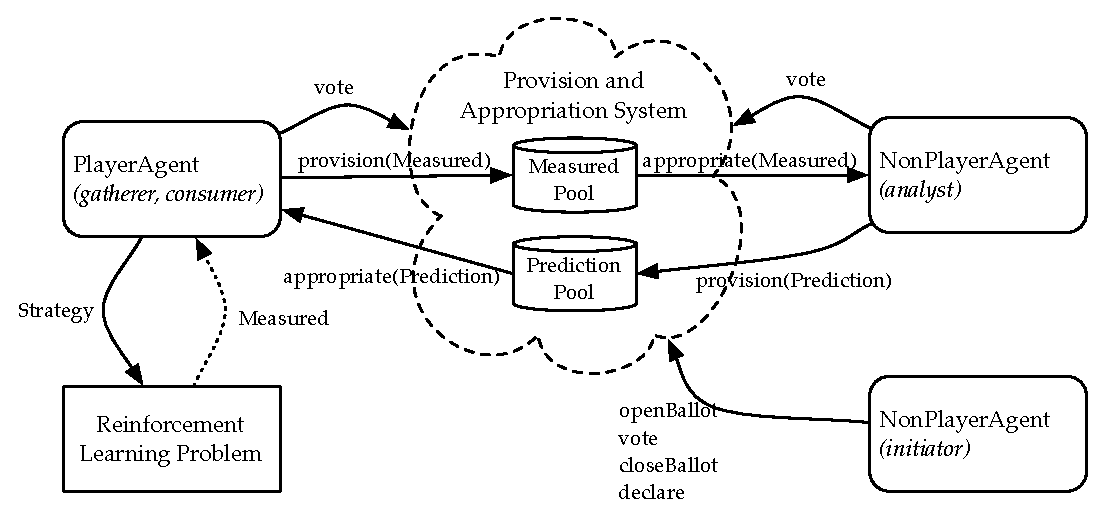
\includegraphics[width=\textwidth]{gfx/simulation_roles}
\caption[Configuration of an institution for reinforcement learning.]{Configuration of an institution for reinforcement learning. Lines show actions and the movement of information in the system. The roles for each agent are displayed in brackets.}\label{fig:simroles}
\end{figure}

\subsection{Agent Implementation}

The agents in this simulation can be classified into two groups: those who are
playing the reinforcement learning game, \texttt{PlayerAgent}s, and those who
are not, \texttt{NonPlayerAgent}s. The former are the \emph{gatherers} and
\emph{consumers} of information, while the latter constitute any other agent
who is involved with the institution in some way. These two groups have
significant overlap in terms of their interactions with the institution,
therefore we propose a behaviour-driven agent implementation where we define
agents with a set of behaviours. These behaviours are independent, but may
read and write shared data to allow for complex behaviours from their
combination. We describe the behaviours we have implemented and how we compose
them.

Our agents have two operating modes which are specified when the agent is created:

\begin{itemize}
\item \emph{Sustainable}---This mode pursues what it deems to be sustainable decisions for the institution. It aims for sustainable outcomes over individual enrichment. However, this does not mean that the agent will sacrifice all his resources on this goal, he will leave the institution if there is no long-term benefit for himself.
\item \emph{Greedy}---This mode pursues individually optimal decisions. It makes self-interested choices whenever possible, in order to maximise acrued rewards.
\end{itemize}

Where applicable we note how a behaviour will be different in each operation mode.

\subsubsection*{Gameplay Behaviour}

This behaviour implements an agent's interaction with the reinforcement
learning problem. This involves choosing a strategy and performing it, as well
as deciding whether to measure the reward gained from this strategy.

There may be multiple \texttt{Prediction}s available, from different
prediction algorithms, in pools which the agent can appropriate from. The
agent may also have its own prediction algorithm to generate strategies.
Therefore the agent employs basic learning to dynamically choose a preferred
source for \texttt{Prediction}s based on the reward gained using this source
in the past.

All agents also have a behaviour to train their own prediction algorithm given the
\texttt{Measured} artifacts available to them. This maybe only self-measured
artifacts, or be ones appropriated from a pool.

Lastly, greedy \texttt{PlayerAgent}s have a behaviour to determine
whether to measure the reward of strategies or not. This behaviour compares the
cost of measuring to the reward given by the institution for provision or
appropriation of this information. If the former is greater then measuring is
disabled for the aforementioned gameplay behaviour.

\subsubsection*{Institutional Behaviours}

The remaining behaviours involve interaction with the institution.
For several of these we are only interested in triggering the behaviour when
the agent is empowered to do a particular action in an institution. For this
we use a \texttt{PowerReactiveBehaviour}. This behaviour reacts to a
particular institutionalised power for an agent, enabling the behaviour when
the agent is empowered, and disabling when they are not. Behaviours that extend
from this class specify the action they require empowerment for, and the
behaviour for each institution where this power exists.

In addition to this use, we define a number of institutional rules which
compel agents to perform actions via an obligation. An
\texttt{InstitutionalBehaviour} is implemented which responds to the presence of obligations
for an agent. The behaviour listens for incoming obligations for an agent and
performs the action as specified. 

\subsubsection*{Provision and Appropriation}

The provision and appropriation behaviours are the primary institution
interaction behaviour for all agents. We implement these as
\texttt{PowerReactiveBehaviour}s for each artifact type. These behaviours are:

\begin{itemize}
\item \texttt{ProvisionMeasuredBehaviour}---When $\B{pow}(\m{provision}(A,\_,M)) = \true$ for an agent $A$ and \texttt{Measured} artifact $M$, agent $A$ will provision any measurements to the institution.
\item \texttt{AppropriatePredictorBehaviour}---When $\B{pow}(\m{appropriate}(A,\_,P)) = \true$ for agent $A$ and \texttt{Prediction} artifact $P$, agent $A$ will \texttt{Request} for any new \texttt{Prediction}s in the pool. Additionally, when this power no longer holds for an institution, any appropriated \texttt{Predictors} from this institution will be removed from the set available to the gameplay behaviour.
\item \texttt{ProvisionPredictorBehaviour}---When $\B{pow}(\m{provision}(A,\_,P)) = \true$ for an agent $A$ and \texttt{Predictor} artifact $P$, agent $A$ will provision its \texttt{Predictor} to the institution, if it has not done so already.
\item \texttt{AppropriateMeasuredBehaviour}---When $\B{pow}(\m{appropriate}(A,\_,M)) = \true$ for agent $A$ and \texttt{Measured} artifact $M$, agent $A$ will \texttt{Request} new \texttt{Measured} artifacts to appropriate from the pool. If there is an appropriation fee for this pool he will limit the number of appropriations such that he does not bankrupt himself.
\item \texttt{PruneMeasuredBehaviour}---When $\B{pow}(\m{remove}(A,\_,M)) = \true$ for agent $A$ and \texttt{Measured} artifact $M$, agent $A$ will \texttt{Prune} old \texttt{Measured} artifacts from the pool. This behaviour aims to keep the number of artifacts in the pool down to avoid incurring high storage costs.
\end{itemize}

\subsubsection*{Role Management}

The \texttt{RoleManagement} behaviour keeps track of the agent's use of
institutional roles. If an agent is no longer utilising the benefits of a role
he can resign in order to avoid incurring costs associated with it. For
example if a \emph{consumer} has appropriated \texttt{Prediction}s from
multiple institutions, but is only using one, he can \texttt{Resign}
membership of the other institutions with no loss of his ability to
appropriate from the preferred \texttt{Prediction}s.

\subsubsection*{Voting}

Finally, agents' \texttt{VoteBehaviour} specifies how they will vote when they
are empowered to vote on a ballot. It has modules for each ballot they may
vote on. Agents are given limited information with which to decide how to
vote. They do not have information about how other agents are performing, and
therefore must decide based on purely their own performance and operating mode. The exception to
this rule is that they can also see the public information of the institution
in order to judge how to set subscription fees. 

In our institution implementation we have implemented two issues we may have collective
choice on: subscription fees and appropriation fees. We have separate voting
behaviour for each. Both votes are done by preference list, where the
candidates are the possible absolute values for these fees.

Firstly, the subscription fee vote strategy varies based on the agent's
operating mode, and whether they occupy the role of \emph{initiator} or not:

\begin{itemize}
\item If the agent is sustainable, they look at the current profit margin of the institution and chose a subscription value which will lead to the institution breaking even. Preferences are chosen by calculating a projected balance for the institution in the future, based on current conditions.
\item If the agent is greedy and is in the \emph{initiator} role, they aim to extract a high fee to make the institution profitable while not so high as to make other agents leave their roles.
\item If the agent is greedy and must pay the fee, they vote for the lowest possible fee.
\end{itemize}

The algorithm for agents to generate these preferences is given in \autoref{alg:subvote}.

% \begin{algorithm}
% 	\SetKwFunction{Map}{map}\SetKwFunction{Abs}{abs}
% 	\SetKwFunction{Sorted}{sorted}\SetKwFunction{Zip}{zip}

% 	currentFee $\leftarrow$ Current subscription fee \\
% 	profit $\leftarrow$ Current Institution profit \\
% 	balance $\leftarrow$ Current Institution balance \\
% 	S $\leftarrow$ Set of possible subscription fee choices \\
% 	nPayers $\leftarrow$ Number of agents currently obligated to pay this fee \\
% 	l $\leftarrow$ Time window over which to make balance estimation \\
% 	\BlankLine
% 	\Begin{
% 	\uIf{profile == SUSTAINABLE}{
% 	baseProfit $\leftarrow$ profit - currentFee * nPayers \\
% 	\ForEach{f in S}{
% 		projections[f] $\leftarrow$ \Abs{balance + l * (baseProfit + f * nPayers)}
% 	}
% 	preferences $\leftarrow$ List of preferences from $S$, sorted by projections \\
% 	}\ElseIf{profile == PROFITABLE}{
% 		\uIf{initiator}{
% 			targetSub $\leftarrow$ $0.7$ - measuringCost \\
% 			\ForEach{f in S}{
% 				diffs[f] $\leftarrow$ \Abs{targetSub - f}
% 			}
% 			preferences $\leftarrow$ List of preferences from $S$, sorted by diffs \\
% 		}\ElseIf{payer}{
% 			preferences $\leftarrow$ List of preferences from $S$, sorted in ascending order \\
% 		}
% 	}
% 	\Return preferences
% 	}
% 	\caption{Subscription voting algorithm.}\label{alg:subvote}
% \end{algorithm}

\begin{pseudocode}[label=alg:subvote,caption={Subscription voting algorithm.}]
currentFee $\leftarrow$ Current subscription fee
profit $\leftarrow$ Current Institution profit
balance $\leftarrow$ Current Institution balance
S $\leftarrow$ Set of possible subscription fee choices
nPayers $\leftarrow$ Number of agents currently obligated to pay this fee
l $\leftarrow$ Time window over which to make balance estimation
begin
	switch profile do
		case "SUSTAINABLE"
			baseProfit $\leftarrow$ profit - currentFee * nPayers
			foreach f in S do
				projections[f] $\leftarrow$ abs(balance + l * (baseProfit + f * nPayers))
			preferences $\leftarrow$ List of preferences from $S$, sorted by projections
		end
		case "GREEDY"
			if initiator then
				targetSub $\leftarrow$ 0.7 - measuringCost
				foreach f in S do
					diffs[f] $\leftarrow$ abs(targetSub - f)
				preferences $\leftarrow$ List of preferences from $S$, sorted by diffs
			else if payer then
				preferences $\leftarrow$ List of preferences from $S$, sorted in ascending order
			end
		end
	end
	return preferences
end
\end{pseudocode}

The appropriation fee voting strategy varies based on whether the agent is a
beneficiary of the fee, a payer, or if they are an initiator. There are
also different strategies for sustainable and greedy operating modes.
Generally, these strategies determine whether to increase, decrease, or keep
the same subscription fee based on their current profit and a range where they
deem their profit acceptable:

\begin{itemize}
\item Greedy beneficiaries chose to increase the fee if their profit is too low;
\item Sustainable beneficiaries increase or decrease the fee depending on whether they are making too little or too much profit respectively, or keep it the same if it is within this range;
\item Greedy payers simply vote for the minimum possible fee;
\item Sustainable payers employ the reciprocal strategy to sustainable beneficiaries and;
\item Initiators simply select an optimal balance between pool fees (which we determine from the first experiments).
\end{itemize}

The algorithm for agents to generate these preferences is shown in \autoref{alg:appfeevote}.

% \begin{algorithm}
% 	\SetKwFunction{Map}{map}\SetKwFunction{Abs}{abs}
% 	\SetKwFunction{Sorted}{sorted}\SetKwFunction{Zip}{zip}

% 	$c$ $\leftarrow$ Current appropriation fee \\
% 	$S$ $\leftarrow$ Set of possible appropriation fee choices \\
% 	$b$ $\leftarrow$ Current balance of the agent,
% 	$p$ $\leftarrow$ Current profit made by the agent \\
% 	\BlankLine
% 	\Begin{
% 	\uIf{beneficiary of fee}{
% 		\Switch{profile}{
% 			\Case{PROFITABLE}{
% 				\lIf{$p < 0.1$}{$r \leftarrow c + 0.1$}
% 				\lElseIf{$p < 1$}{$r \leftarrow c + 0.05$}
% 				\lElse{r $\leftarrow$ c}
				
% 			}
% 			\Case{SUSTAINABLE}{
% 				\lIf{$p < -0.5$ or $b < 0$}{$r \leftarrow c + 0.1$}
% 				\lElseIf{$p > 0.8$}{$r \leftarrow c - 0.05$}
% 				\lElseIf{$p > 1$}{$r \leftarrow c - 0.1$}
% 				\lElseIf{$p < 0.1$}{$r \leftarrow c + 0.05$}
% 				\lElse{r $\leftarrow$ c}
% 			}
% 		}
% 	}\ElseIf{payer of fee}{
% 		\Switch{profile}{
% 			\Case{PROFITABLE}{
% 				\Return List of preferences from $S$, sorted in ascending order \\
% 			}
% 			\Case{SUSTAINABLE}{
% 				\lIf{$p < -1$}{$r \leftarrow c - 0.1$}
% 				\lElseIf{$p <= 0.1$}{$r \leftarrow c - 0.05$}
% 				\lElseIf{$p > 1$}{$r \leftarrow c + 0.05$}
% 				\lElseIf{$p > 2$}{$r \leftarrow c + 0.1$}
% 				\lElse{r $\leftarrow$ c}}
% 		}
% 	}\ElseIf{initiator}{
% 		\lIf{measuredPool}{$r \leftarrow \m{measuringCost}$}
% 		\lElse{$r \leftarrow 0.075 + (9 * \m{measuringCost} / 10)$}
% 	}
% 	\ForEach{f in S}{
% 		$d[f]$ $\leftarrow$ \Abs{r - f}
% 	}
% 	preferences $\leftarrow$ List of preferences from $S$, sorted by $d$ \\
% 	\Return{preferences}
% 	}
% 	\caption{Appropriation fee voting algorithm.}\label{alg:appfeevote}
% \end{algorithm}

\begin{pseudocode}[label=alg:appfeevote,caption={Appropriation fee voting algorithm.}]
c $\leftarrow$ Current appropriation fee
S $\leftarrow$ Set of possible appropriation fee choices
b $\leftarrow$ Current balance of the agent,
p $\leftarrow$ Current profit made by the agent
begin
	if beneficiary of fee then
		switch profile do
			case "GREEDY"
				if p < 0.1 then r $\leftarrow$ c + 0.1
				else if p < 1 then r $\leftarrow$ c + 0.05
				else r $\leftarrow$ c
			end
			case "SUSTAINABLE"
				if p < -0.5 or b < 0 then r $\leftarrow$ c + 0.1
				else if p > 0.8 then r $\leftarrow$ c - 0.05
				else if p > 1 then r $\leftarrow$ c - 0.1
				else if p < 0.1 then r $\leftarrow$ c + 0.05
				else r $\leftarrow$ c
			end
		end
	else if payer of fee then
		switch profile do
			case "GREEDY"
				return List of preferences from S, sorted in ascending order
			end
			case "SUSTAINABLE"
				if p < -1 then r $\leftarrow$ c - 0.1
				else if p <= 0.1 then r $\leftarrow$ c - 0.05
				else if p > 1 then r $\leftarrow$ c + 0.05
				else if p > 2 then r $\leftarrow$ c + 0.1
				else r $\leftarrow$ c
			end
		end
	else if initiator then
		if measuredPool then r $\leftarrow$ measuringCost
		else r $\leftarrow$ 0.075 + (9 * measuringCost / 10)
	end
	foreach f in S do
		d[f] $\leftarrow$ abs(r - f)
	end
	preferences $\leftarrow$ List of preferences from S, sorted by d
	return preferences
end
\end{pseudocode}

% In self-org or here?

\subsubsection*{Behavioural Composition}

Due to the power-reactive nature of most of the institutional behaviours we
can include them in all agents, and they will lie dormant if they are not
applicable to the roles the agent occupies in the institution. This means that
the differences between agents are determined by the allocation of 
non-institutional behaviours, their operating mode and the initial
\texttt{Predictor}. We define agents for each of the participatory sensing
roles as follows:

\begin{itemize}
\item \emph{Gatherer}/\emph{consumer} agents, which use gameplay and predictor training behaviours;
\item \emph{analyst} agents, which use predictor training behaviour, and will have a better \texttt{Predictor} than gatherers; and
\item an \emph{Initiator} agent, which uses only institutional behaviours.
\end{itemize}

\section{Evaluative Criteria}

In our analysis of participatory sensing using the \ac{IAD} framework, we finished by
discussing five evaluative criteria which can be used to assess the efficacy
of a knowledge commons. We revisit these within the context of our model to
obtain quantitative measures of system performance. We can then use these as
tools for objective comparison of different approaches to managing
information and knowledge resources.

We define these criteria in the context of our experimental model. We then
describe how we use these criteria in our simulations in order to present
comparisons between simulation runs.

\subsection{Definition}

\begin{enumerate}
\item \emph{Increase in knowledge} evaluates the extent to which the system has
generated new knowledge. In our model, reward gained is a direct measure of the
quality of knowledge. Therefore, we can give a metric of the knowledge generated
by the system as the sum of all agent accrued rewards.

The knowledge generated in a time-step $t$, $\mathcal{K}(t)$, can therefore be expressed as the sum of the rewards accrued by all agents in the system within this time-step:
\begin{equation*}
\mathcal{K}(t) := \sum_{\mathit{ag}\in A} \mathit{rewardAccrued}(\m{ag}, t)
\end{equation*}
where $A$ is the set of all agents in the system.

\item \emph{Sustainability} measures whether a system endures in the long term.
This can be simply measured by testing whether the institution has not shut down 
due to bankruptcy after a fixed period of time.

We can express this as whether the institutional account, which pays for facility costs, is positive at a time-step $t$. This function $\mathcal{S}(i,t)$ returns a Boolean representation of whether the institution $i$ has endured until time $t$:
\begin{equation*}
\mathcal{S}(i,t) := \left( \sum_{t^\prime=0}^{t} \mathit{rewardAccrued}(i, t^\prime)\right) > 0
\end{equation*}
Where $i$ is the institutional account, such that $\mathit{rewardAccrued}(i, t)$ returns the rewards received for the running of the institution at time $t$, minus the cost of running it.

\item \emph{Participation standards} measures the level of participation within the 
institution. As our agents are implemented such that they will resign roles they 
no longer need, the number of occupied roles is a good measure of participation.

Thus, we express this metric, $\mathcal{P}(i,t)$ as the number of roles occupied in the institution $i$ at the time $t$:
\begin{align*}
\mathcal{P}(i,t) &:= \sum_{\m{ag}\in A,r\in R} x \\
\text{where\ \ } x &= \begin{cases} 1 & \text{if} \holdsAt(\m{role\_of}(\m{ag},i,r),t) = \true \\
0 & \text{otherwise} \end{cases}
\end{align*}
Where $A$ is the set of agents and $R$ is the set of possible roles.

\item \emph{Efficiency} determines the economic cost of the system relative to its productive output. In this case the cost is purely measured by facility cost and the output is the accumulated rewards.

We express this metric by measuring the fractional proportion of output used on facility costs, and subtracting this from 1. This expression can be written as follows:
\begin{equation*}
\eta(i,t) := \frac{\sum_{t^\prime=0}^{t} \mathcal{K}(t^\prime)}{\sum_{t^\prime=0}^{t} \left( \mathcal{K}(t^\prime) + \m{facilityCost}(i,t^\prime) \right)} 
\end{equation*}
Where $\mathcal{K}(t)$ is accumulated knowledge, from metric 1, and $\m{facilityCost}(i,t)$ returns the cost of the facility for institution $i$ in time-step $t$.

\item \emph{Equity} measures whether agents the are compensated according to
their efforts.  Given that all agents have the potential to achieve the same,
we can expect that an equitable system will result in all agents achieving the
same total rewards. Therefore the equity can be measured as the standard
deviation of the set of all agents' accrued rewards. 

This is expressed by $\mathcal{E}(t)$ which constructs the set of accrued rewards for all agents for the time window $0-t$, then calculates the standard deviation over this set:
\begin{equation*}
\mathcal{E}(t) := \sigma ( S_t ) \text{, where } S_t = \left\{ \mathit{ag}\in A : \sum_{t^\prime=0}^{t} \mathit{rewardAccrued}(\m{ag}, t^\prime) \right\}
\end{equation*}

In order to match the other
criteria, which all have the property that a higher value represents better
performance, we instead measure the ratio of the standard deviation and mean,
which gives a unitless measure of inequity, then subtract it from $1$. This
gives a measure where $1$ means everyone received the same rewards, values less than
this indicate increasing inequity:
\begin{equation*}
\mathcal{E}^\prime(t) := 1 - \frac{\sigma ( S_t )}{\overline{S_t}}
\end{equation*}

\end{enumerate}

% TODO usage?

\subsection{Presentation in the results}\label{sec:criteriapres}

The criteria which we have defined can all be measured at various time-points
in the simulation. For the purposes of our simulations we use the criteria for comparison between simulation runs, to determine if one run is `better' than another. We measure the defined criteria as follows:

\begin{itemize}
\item \emph{Increase in knowledge} is measured as the cumulative sum over the whole simulation time: $\sum_{t=0}^{t_{\m{max}}} \mathcal{K}(t)$.
\item \emph{Sustainability} is measured at the end of the elapsed simulation time, thus we measure $\mathcal{S}(i,t_{\m{max}})$.
\item \emph{Participation Standards} are measured by comparing the institution membership at the start and end of the simulation: $\frac{\mathcal{P}(i,t_{\m{max}})}{\mathcal{P}(i,0)}$
\item \emph{Efficiency} is measured at the end of simulation time: $\eta(i, t_{\m{max}})$
\item \emph{Equity} is also measured at the end of simulation time: $\mathcal{E}^\prime(t_{\m{max}})$
\end{itemize}

When comparing a group of simulations we also normalise the total rewards
(increase in knowledge) by dividing all values by the largest in the set. This
therefore leads to all criteria being specified in the range $[0,1]$.
Averaging the normalised criteria for each simulation gives a total score,
representing performance across all criteria.

When performing parameter sweeps we display the resulting evaluative criteria
in heatmaps. These visualise where optimal parameter configurations lie. Our
heatmaps show four individual maps, showing normalised participation
standards, increase in knowledge, equity, and the total score over all 5
criteria. 

% We omit individual maps for sustainability and efficiency to avoid
% duplicating information unnecessarily. The former follows the same trend as
% participation standards. In the sets of simulations we compare, environmental
% conditions remain constant, thus facility costs will be a constant. Therefore,
% efficiency will follow the same trend as increase in knowledge.

\section{Experimental Agenda and Simulation Results}

We now combine the three components from the previous section: the reinforcement learning problem, the institution for provision and
appropriation of artifacts for this problem, and the agent implementations as
described to create our computer model of participatory sensing. We perform
controlled experimentation with this model in order to answer the following question.
How can governance be provisioned for participatory sensing?

In \autoref{ch:kc} and \autoref{sec:iad} we outlined the problem of supply of
institutions. This problem is the difficulty in supplying an effective institution to
a \ac{CPR} problem. Here we have done much of the work in specifying an
institution which defines boundaries and provides scope for dynamic
appropriation and provision rules depending on conditions. However, this is no
guarantee of a `good' outcome. 

In our first round of experiments we investigate
the specification space of our system to determine whether a trade-off between
our evaluative criteria can be found, and how the system's equilibrium changes
under different conditions.

In the second set of experiments we take this further, and test our hypothesis
that appropriate enfranchisement of agents can lead to a good outcome,
according to our evaluative criteria. To do this we exploit the flexibility of
our institutional specification to deploy centralised, market-based, and
collective governance in simulation. Through comparison of these three
paradigms we can draw parallels with our participatory-sensing review and the
problems we outlined in \autoref{ch:kc}.

% We model a participatory sensing problem as a reinforcement learning problem (See Sutton \& Barto). Policies are knowledge artifacts, which can be appropriated and used to chose actions. Agents are able to measure directly the reward from an action when performing it. Their aim is to maximise rewards over time by training a better policy. All agents play the same game, so policies and measurements are useful for everyone, and one agent's measurements can be used to train another's policy.

% As policies will improve with more information, the best strategy for agents will be to pool their information and knowledge together. 
% Therefore, by forming an institution around this information and knowledge, everyone should be able to achieve a better utility overall.

%The simulation is set up as a symmetric participatory sensing problem. This is a problem where agents are playing a repeated game where, in each round, a strategy played by the agent yields a reward. Agents are able to measure their previous rewards. They aim to maximise their reward over time by learning the best strategy to choose. As all agents are playing the same game this learning can obviously be improved by gathering together this information. Additionally not all agents will have the knowledge or capability to do this learning themselves. 

% The institution is constructed as a provision and appropriation system with two pools. One for information as gathered by the learning agents, and the other for knowledge provided by analysts. This problem is symmetric as each group of agents will provision to one pool and appropriate from the other---learning agents provision information and appropriate knowledge and appropriate information and provide knowledge---thus they are also dependant on each other. If the institution is unsatisfactory for one group and they leave it will quickly become unsatisfactory for the others too.

% The utility generated from the learning problem acts as the only external input of value into the system, while paying for facility costs is the only way of value flowing out of the system. All other transactions are endogenous. There is also a possibility, as seen in many real-world participatory sensing systems, of other exogenous rewards from ownership of a data-set, however we do not simulate this.

% \subsection{Rewarding Knowledge}

% In order to model the additive value of information when combined for learning we use an artificial reward function which gives a utility proportional to the quality of policy used to chose an action. The quality of a policy is defined as the number of information samples over a time window from the current time:

% A policy is a tuple containing a set of data samples: $P = <S>$. A predictor can recommend an action for an agent: $\mathit{selectAction}(P,t) \rightarrow s_t$. Using this action then yields a reward: $u(s_t) = \sum_t^{t-W} \frac{|S_t|}{W*N}$ where $W$ is a time-window size for which information is useful and $N$ is maximum number of samples possible in one time-step. This function returns a value between 0 and 1.

%\section{Experiments}

\subsection{The Problem of Supply}\label{sec:supply}

\subsubsection*{Experimental Setup}

In these experiments we investigate how a static institution (one without
coll\-ective-choice to change its parameters during operation) performs
according to our evaluative criteria. We construct an institution as follows:

\begin{itemize}
\item Facility costs shared between \emph{consumer} and \emph{analyst} roles.
\item Configurable fees to pay providers when their artifacts are appropriated. This fee is paid by the appropriators. These fees remain constant throughout the simulation.
\end{itemize}

We configure a population of agents as follows:

\begin{itemize}
\item 10 \texttt{PlayerAgent}s in \emph{sustainable} mode and occupying \emph{gatherer} and \emph{consumer} roles. These agents are given no \texttt{Predictor} initially.
\item One \texttt{NonPlayerAgent} in the \emph{analyst} role. This agent is given a \texttt{Predictor}.
\item One \texttt{NonPlayerAgent} in the \emph{initiator} and \emph{manager} roles to perform institution administration tasks.
%\item One \texttt{PlayerAgent} with no roles in the institution and with the same \texttt{Predictor} as the analyst. This player acts as a benchmark for independent vs. cooperative play.
\end{itemize}

We run parameter sweeps to investigate how the pool appropriation fees
affect the evaluative criteria. We test the cost to appropriate an action from
\texttt{Predictor} in the range $0-1$ in intervals of $0.1$, and the cost to
appropriate \texttt{Measured} information in the range $0-0.5$ in $0.02$
intervals. For each parameter set we simulate 200 time-steps. The simulations
are deterministic, so we do not require repeats.

We create a set of scenarios with varying environmental conditions, as shown
in \autoref{tab:scenarios}. We have two facility cost profiles:
\emph{flexible} costs, where each provision and appropriation action costs
$0.1$; and \emph{fixed} costs, where the facility costs a fixed fee of $2.0$ per
time-step. We also test with no cost for measuring, and with a small cost of
$0.1$. Finally, we test the introduction of three \texttt{PlayerAgent}s who are in
\emph{greedy} mode, replacing three of the sustainable agents. These scenarios aim to test increasingly difficult environmental conditions, and how they affect the performance, in particular participatory levels and sustainability of the institution.

The first scenario has low facility costs, no cost of
measuring, and all agents behave in a way which aims to lead to
sustainability. Therefore the institution simply needs to cover the facility
costs allocate rewards suitability to ensure that all agents can effectively
contribute.

The second scenario introduces a measuring cost into the previous
configuration. This tests whether the institutional configuration is able to
handle the additional cost incurred for the gathering of information.

The third scenario modifies the second configuration, changing the nature of
the facility costs. This aims to test if the nature of these costs will affect
the system performance, even when the total facility costs over the course of
the simulation will not be significantly different.

Finally, the fourth configuration replaces some sustainable agents with greedy ones, with the conditions
as in scenario 2. This will test firstly, whether greedy agents will negatively
affect the system as a whole, and secondly, whether greed is beneficial for
the individual, in terms of higher accrued rewards.

In this experiment we aim to firstly determine the effect of the values of
the fees charged for different artifacts in the institution, and secondly, how
these effects change under differing environmental conditions.

% We also alter environmental conditions, to create different scenarios, as follows:

% \begin{enumerate}
% \item Measuring cost: $\{0, 0.1\}$,
% \item Facility costs: \emph{flexible} costs, where each provision and appropriation action costs $0.1$; and \emph{fixed} costs, where the facility costs a fixed fee of $2$ per time-step.
% \item Non-compliant agents: the number of the 10 \texttt{PlayerAgent}s who are in \emph{non-compliant} mode.
% \end{enumerate}

\begin{table}
\centering
\caption{Conditions for static simulation scenarios.}\label{tab:scenarios}
\begin{tabular}{c||c|c|c}
Scenario & Facility cost & Measuring cost & Greedy agents \\
\hline
1 & flexible & 0 & 0 \\
2 & flexible & 0.1 & 0 \\
3 & fixed & 0.1 & 0 \\
4 & flexible & 0.1 & 3 \\
\end{tabular}
\end{table}

\subsubsection*{Results}

\begin{table}
\centering
\caption[Evaluation of institution configurations in scenario 1.]{Evaluation of institution configurations in scenario 1. Shows only best and worst five parameter combinations.}\label{tab:static0}
\begin{tabular}{rr|rcrrr|c}
Meas. & Pred. & Rewards & Endures? & Partic. & Efficiency & Equity & Total \\
\hline
0.22 & 0.3 & 1287 & Yes. & 100.0\% & 76.4\% & 0.97 & 0.996 \\
0.12 & 0.2 & 1273 & Yes. & 100.0\% & 76.2\% & 0.97 & 0.994 \\
0.32 & 0.4 & 1284 & Yes. & 100.0\% & 76.4\% & 0.96 & 0.994 \\
0.02 & 0.1 & 1265 & Yes. & 100.0\% & 76.1\% & 0.97 & 0.994 \\
0.42 & 0.5 & 1274 & Yes. & 100.0\% & 76.2\% & 0.95 & 0.990 \\
\vdots & \vdots & \vdots & \vdots & \vdots & \vdots & \vdots & \vdots \\
0.0 & 0.8 & -44 & Yes. & 13.0\% & 0.0\% & 0.0 & 0.274 \\
0.0 & 0.7 & -44 & Yes. & 13.0\% & 0.0\% & 0.0 & 0.274 \\
0.0 & 0.4 & -44 & Yes. & 13.0\% & 0.0\% & 0.0 & 0.274 \\
0.0 & 0.6 & -45 & Yes. & 13.0\% & 0.0\% & 0.0 & 0.274 \\
0.0 & 0.5 & -45 & Yes. & 13.0\% & 0.0\% & 0.0 & 0.274 \\
\end{tabular}
\end{table}

\autoref{fig:static0} shows heatmaps for the first scenario\footnote{A description of how data is displayed in the heatmaps was given in \autoref{sec:criteriapres}}: flexible
facility costs and no measuring cost. As can be seen also in
\autoref{tab:static0}, there are several configurations which all give high
scores. Firstly, the participation standards graph shows that there are many
viable configurations which will keep all agents participating in the
institution, however comparing to the total knowledge plot we see that several of
these lead to a less optimal outcome. Equity can be seen to peak at several
equilibria when the correct balance between \texttt{Measured} and
\texttt{Prediction} fees is achieved. When the criteria are aggregated into a
total score, equity is to be the differentiating factor between the best
performing configurations, causing those equilibria to be visible in the total
score too.

\begin{figure}
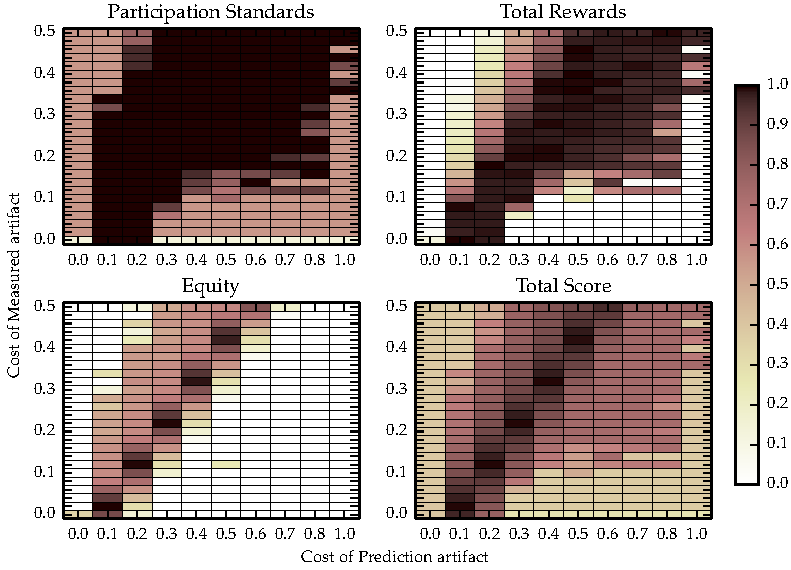
\includegraphics{gfx/kc/static_0.pdf} 
\caption[Comparison of scores between configurations in scenario 1.]{Comparison of scores between configurations in scenario 1. Darker/higher is better.}\label{fig:static0}
\end{figure}

Introducing a measuring cost into the scenario significantly reduces the
number of enduring configurations, as shown in \autoref{fig:static1}.
Additionally, the optimal equilibria are slightly shifted compared to in the
previous scenario.

\begin{figure}
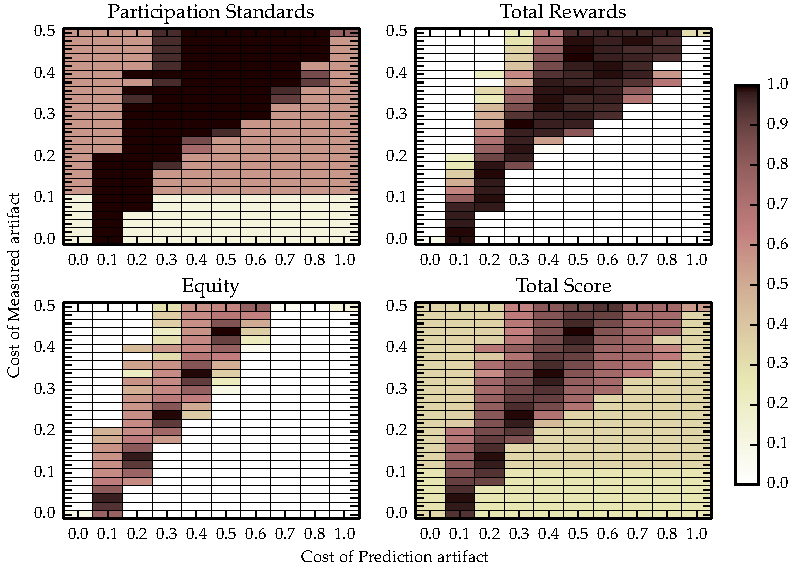
\includegraphics{gfx/kc/static_1.pdf} 
\caption[Comparison of scores between configurations in scenario 2.]{Comparison of scores between configurations in scenario 2. Darker/higher is better.}\label{fig:static1}
\end{figure}

When facility costs are set at a fixed rate, we see that the configurations
which lead to endurance and high participation are further reduced, shown in
\autoref{fig:static_highfixed_1}. However, the facilities are only marginally
dearer overall, as we can see from the efficiency given in
\autoref{tab:staticfixed1}.

\begin{table}
\centering
\caption[Evaluation of simulation performance in scenario 3.]{Evaluation of simulation performance in scenario 3. Shows only best ten parameter combinations.}\label{tab:staticfixed1}
\begin{tabular}{rr|rcrrr|c}
Meas. & Pred. & Rewards & Endures? & Partic. & Efficiency & Equity & Total \\
\hline
0.44 & 0.5 & 1084 & Yes. & 100.0\% & 73.1\% & 0.96 & 0.997 \\
0.34 & 0.4 & 1064 & Yes. & 100.0\% & 72.7\% & 0.97 & 0.993 \\
0.24 & 0.3 & 1077 & Yes. & 100.0\% & 72.9\% & 0.95 & 0.992 \\
0.14 & 0.2 & 1063 & Yes. & 100.0\% & 72.7\% & 0.95 & 0.989 \\
0.04 & 0.1 & 1064 & Yes. & 100.0\% & 72.7\% & 0.94 & 0.987 \\
0.42 & 0.5 & 1084 & Yes. & 100.0\% & 73.0\% & 0.91 & 0.982 \\
0.02 & 0.1 & 1083 & Yes. & 100.0\% & 73.0\% & 0.9 & 0.98 \\
0.32 & 0.4 & 1095 & Yes. & 100.0\% & 73.3\% & 0.89 & 0.979 \\
0.12 & 0.2 & 1085 & Yes. & 100.0\% & 73.1\% & 0.9 & 0.979 \\
0.22 & 0.3 & 1078 & Yes. & 100.0\% & 72.9\% & 0.88 & 0.974 \\
\vdots & \vdots & \vdots & \vdots & \vdots & \vdots & \vdots & \vdots \\
\end{tabular}
\end{table}

\begin{figure}
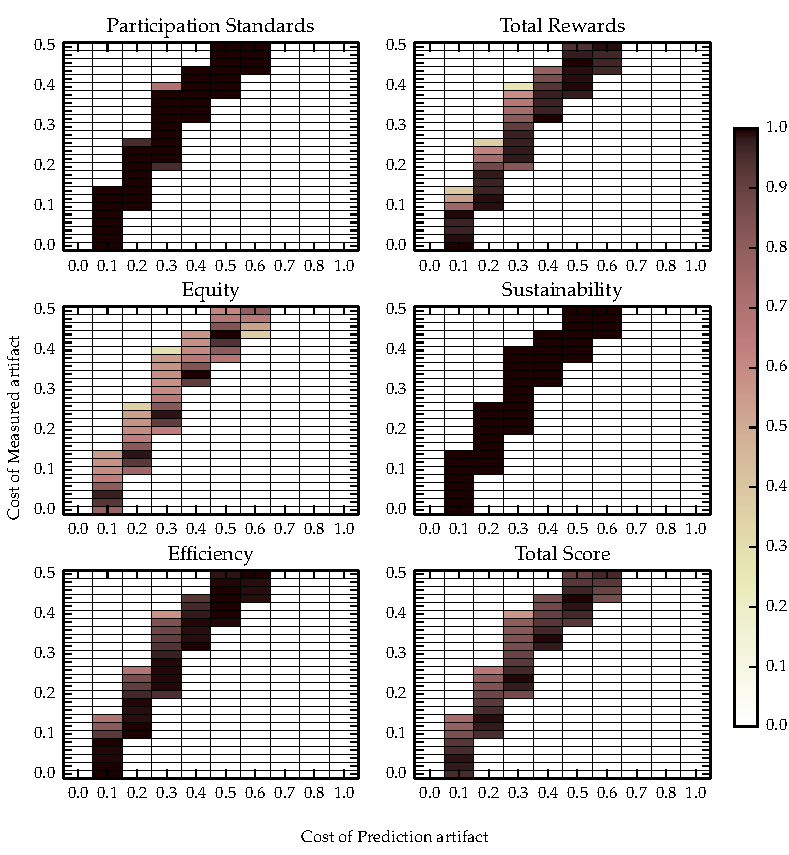
\includegraphics{gfx/kc/static_highfixed_1.pdf} 
\caption[Comparison of scores between configurations in scenario 3.]{Comparison of scores between configurations in scenario 3. Darker/higher is better.}\label{fig:static_highfixed_1}
\end{figure}

Finally, we test the effect of the introduction of greedy agents into
the system. \autoref{fig:static3nc} shows the results for a system with 3 greedy agents. Here participation levels and utility are reduced when the
reward for provision of \texttt{Measured} artifacts is less than $0.1$. This is
due to the greedy agent behaviour to not measure when the reward is
less than the cost.

\begin{figure}
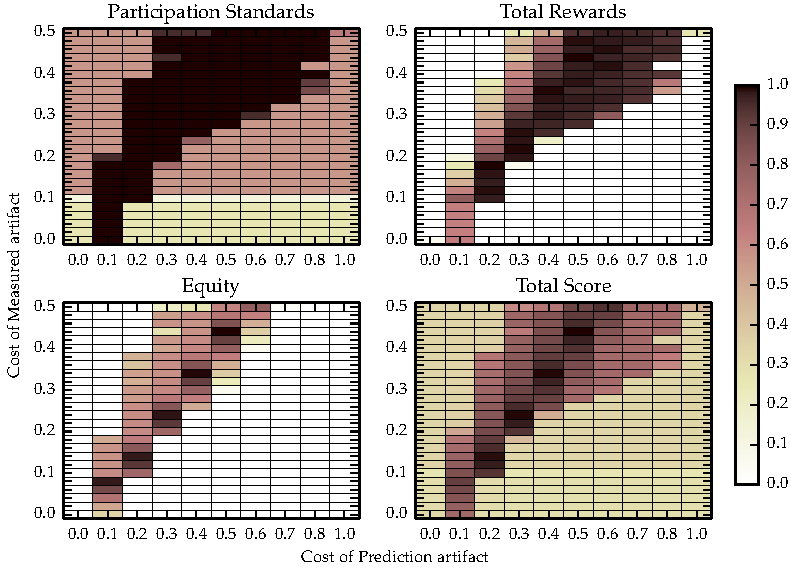
\includegraphics{gfx/kc/static_1_3nc.pdf} 
\caption[Comparison of scores between configurations in scenario 4 (3 greedy agents).]{Comparison of scores between configurations in scenario 4 (3 greedy agents). Darker/higher is better.}\label{fig:static3nc}
\end{figure}

\subsubsection*{Discussion}

From these experiments we see that, firstly, if the right balance between
costs and benefits for agents in each role is not achieved, we will not get
high participation standards. In the case when the \texttt{PlayerAgent}s' costs
outweigh their rewards they will choose to stop appropriating predictions, and
then resign their \emph{consumer} role. Similarly, if the cost of
\texttt{Measured} artifacts is too high, the \emph{analyst} will no longer be
able to afford to appropriate them all, resulting in sub-optimal
predictions, and lower rewards for everyone.

Secondly, many configurations result in near-optimal accrued rewards; however very
few result in optimal equity. This is because optimal rewards can be achieved
simply by ensuring that all agents provision and appropriate as much as
possible. This is a looser constraint than for equity, which must balance the
allocation of rewards between roles. Optimal equity is only achieved when
the exact balance between fees is achieved to make their rewards converge
over time.

Thirdly, the nature of facility costs can have a significant effect on the
sustainability of the institution. We saw that with fixed costs sustainability
was much more difficult to achieve. At the start of a simulation we find that
rewards are particularly scarce. With flexible institution costs, a reduction
in institutional transactions, for example when agents cannot afford to
appropriate, will result in a lower facility cost, giving the leeway required
to raise enough rewards to appropriate in the next time-step. When costs are
fixed there is the opposite effect, causing struggling institutions to fail.
This leads to the divergence in rewards shown in
\autoref{fig:static_highfixed_1}, where configurations either succeed with
high utility or fail. With dynamic costs we see a larger range of outcomes.

Similarly, greed affects the sustainability of the institution, as
the introduction of free-riders reduces the efficiency of the institution.
However, this free-riding can be easily corrected through the use of an
incentive for the greedy agents to contribute. This incentive is also
non-discriminatory, because sustainable agents also receive it, and its cost can
be easily offset through the cost of appropriating predictions. In
\autoref{fig:static3nc} we see that once the \texttt{Measured} cost is over
$0.1$ the system behaves as with no greediness.

%Finally, when looking at the difference between successful and unsuccessful simulations, we see that ???

% This first set of experiments looks at the problem of provisioning an institution for the problem we have outlined. Despite having a simple game where we can seemingly trivially generate utility, getting together disparate agents to all contribute and keeping it sustainable over the long time requires negotiating several hurdles. 

% We will see these hurdles as we follow the process of building a centralised institution for this problem. This institution has a single agent who acts as a manager for the institution and as complete control over institutional fluents.

% The experimental setup is as follows:
% \begin{itemize}
% \item One institution with information and knowledge pools.
% \item 10 gatherer/consumer agents who are members of the institution.
% \item One analyst agent providing knowledge for the institution.
% \item One initiator agent managing the institution.
% \item One independent agent as a control benchmark. This agent has the same knowledge as the analyst, but only uses self-gathered information.
% \end{itemize}

% \subsubsection{Facility Cost}

% Storing information and knowledge, and other infrastructure required for the institution will incur facility costs. We have two profiles to model facility costs:
% \begin{itemize}
% \item High sunk cost --- A high initial sunk cost (for infrastructure acquisition), followed by a lower fixed cost each time-step ($\mathtt{sunk\_cost}=50$, $\mathtt{fixed\_cost}=1$).
% \item High fixed cost --- No initial sunk cost, higher fixed cost ($\mathtt{sunk\_cost}=0$, $\mathtt{fixed\_cost}=2$).
% \end{itemize}

% We are running simulations over 200 time-steps, so these profiles would correspond to a total incurred cost of 250 and 400 respectively.

% \begin{figure}
% 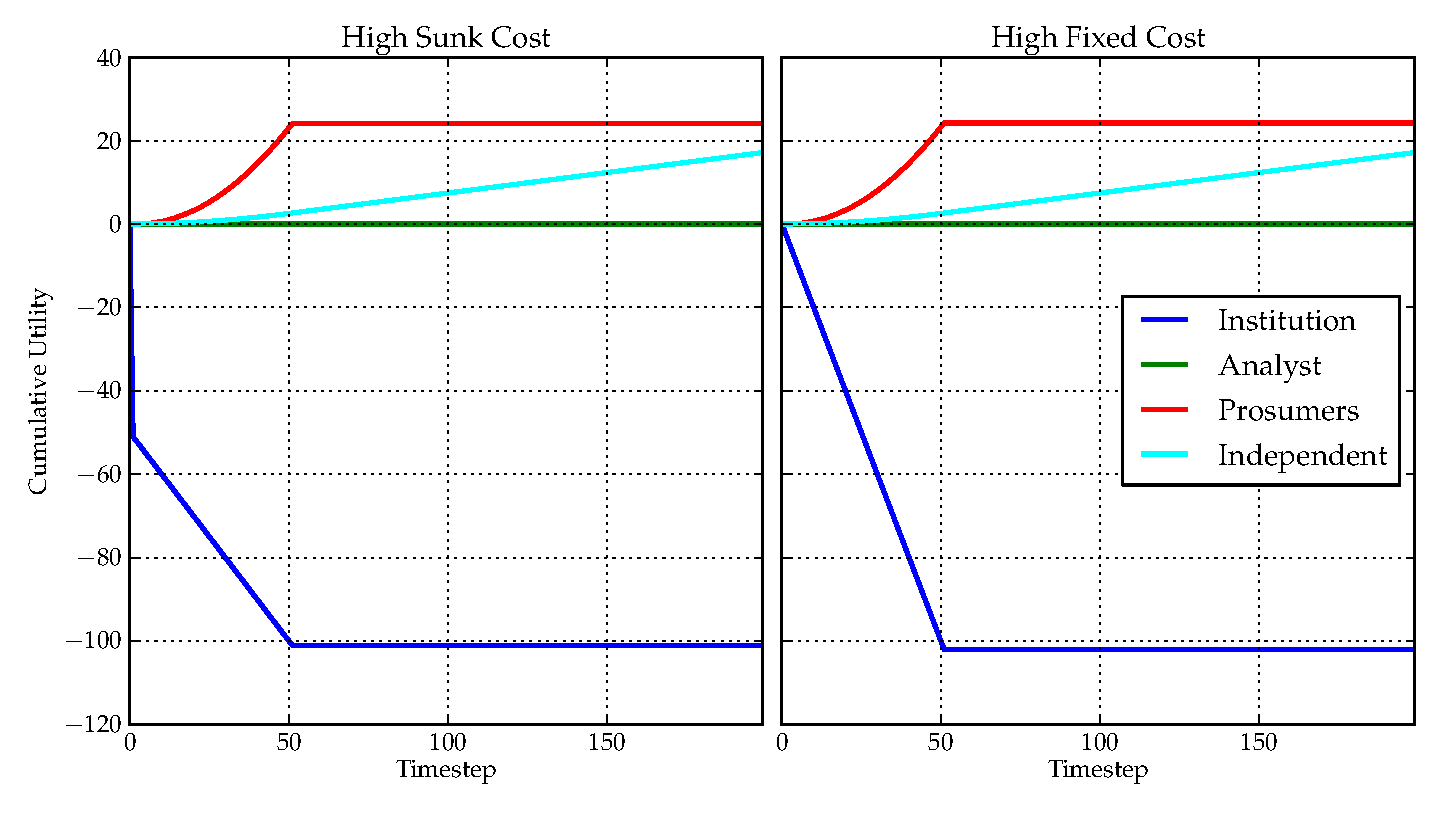
\includegraphics[width=\linewidth]{gfx/kc/facility1v2.pdf} 
% \caption{Cumulative agent utilities over time in basic centralised institution with high--sunk and high--fixed facility profiles.}\label{fig:facility1}
% \end{figure}

% Figure~\ref{fig:facility1} shows the utilities in this scenario. In both cases the institution runs out of resources to pay for facilities after 50 timesteps, at which point the institution ceases to function. As the in-flow of utility into the system (to prosumers) is separate from where the facility is paid for (by the initiator) then the system cannot endure without the charity of the initiator. Therefore without exogenous income for this agent we require a way for prosumers to contribute to the facility costs.

% One method we can use is to have a subscription fee. This is a payment to the institution each timestep which one is occupying a certain role. The level of this fee is determined by the initiator who has the sole power to set its value. 

% \begin{figure}
% 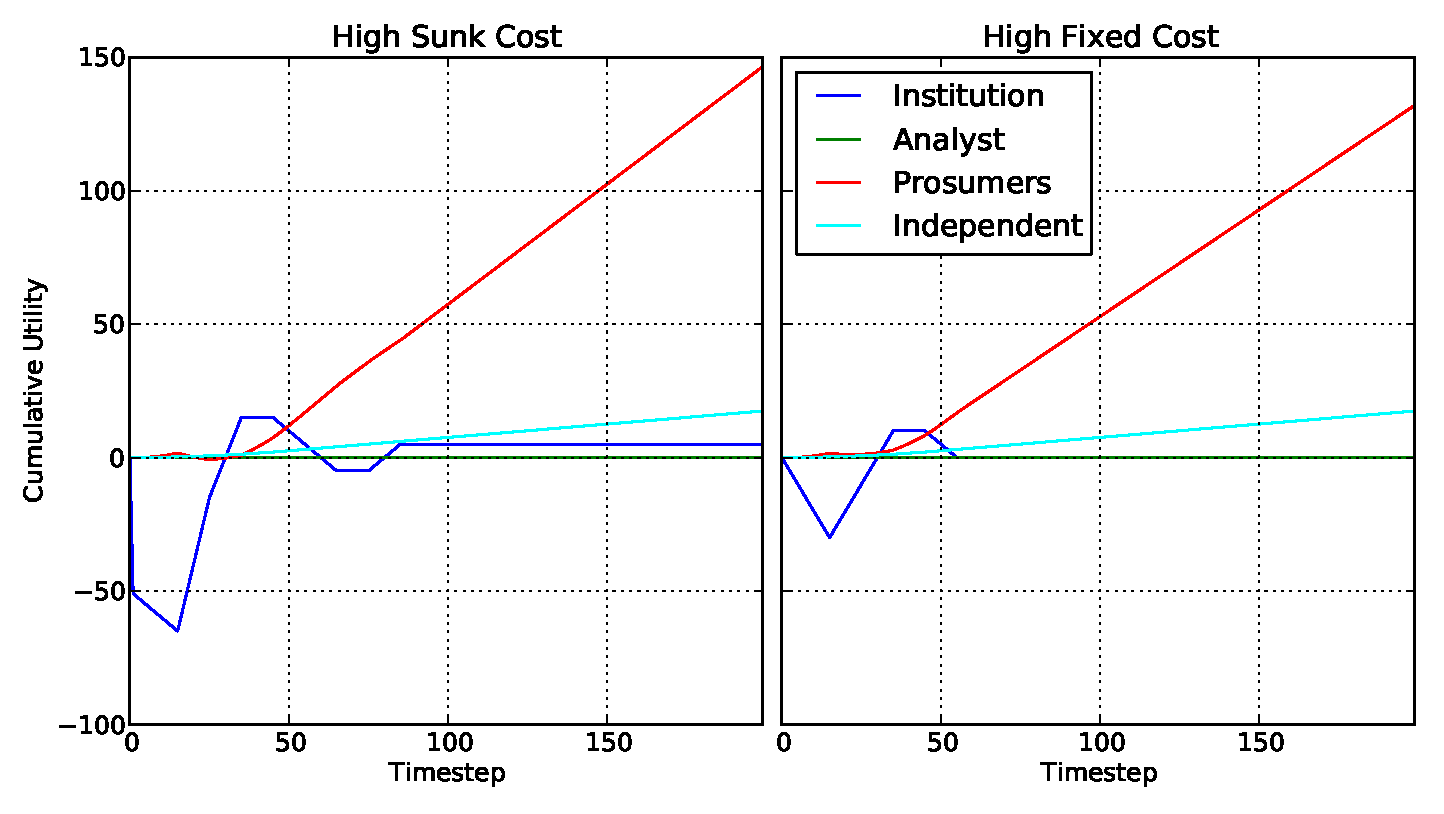
\includegraphics[width=\linewidth]{gfx/kc/facility2.pdf} 
% \caption{Cumulative agent utilities over time in centralised institution using subscription fees with high--sunk and high--fixed facility profiles.}\label{fig:facility2}
% \end{figure}

% Figure~\ref{fig:facility2} shows agent utilities once subscription fees are introduced. The rate dynamically adjusts to ensure that the institution breaks even and that the institution endures. Here we also see the benefit of the institution. Prosumer agents accrue over 7.5 times more than the independent control agent in each case due to having 10 times more data and only small additional overheads.

% \subsubsection{Compensating Analysts}

% Figures~\ref{fig:facility1}~\&~\ref{fig:facility2} from the previous section both show zero utility gained for the analyst agent. However are having to appropriate information and process it in order to generate the knowledge which they provision. Given that this knowledge enables a large increase in reward for the prosumer agents, analysts may expect some remuneration.

% This can be achieved by paying an analyst when knowledge is appropriated. Again the initiator can set the rate for this payment. Table~\ref{tab:analyst1} shows final utilities for agents when a fixed rate of 0.1 per appropriation is set.

% \begin{table}
% \centering
% \begin{tabular}{c|c||c|c}
% Facility Profile & Pay Analysts? & Prosumers & Analyst \\ 
% \hline \hline
% High sunk & no & 142 & 0 \\ 
% \hline 
% High sunk & yes & 127 & 157 \\ 
% \hline 
% High fixed & no & 128 & 0 \\ 
% \hline 
% High fixed & yes & 112 & 144 \\ 
% \end{tabular}
% \caption{Compensation of analysts}\label{tab:analyst1}
% \end{table} 

% \subsubsection{Compensating Gatherers}

% In the previous examples all prosumers always gather information, and always provision it, as there is no cost for them in this process. However in some cases there is likely to be some costs associated with gathering information. In turn this may cause some agents to `free-ride' by not gathering or provisioning information while still receiving the benefits of the institution. Again we can simply introduce a payment for provision or appropriation of this information.

% \begin{table}
% \centering
% \begin{tabular}{c|c|c||c|c|c}
% Facility Profile & Pay Gatherers? & No. Greedy & Compliant & Non-compliant & Analyst \\ 
% \hline \hline
% High sunk & no & 2 & 74 & 93 & 157 \\ 
% \hline 
% High sunk & no & 5 & -8 & -1 & -8 \\ 
% \hline
% High sunk & yes & 2 & 91 & 92 & -4 \\ 
% \hline 
% High sunk & yes & 5 & 92 & 91 & -4 \\ 
% \hline  
% High fixed & no & 2 & 61 & 81 & 144 \\ 
% \hline 
% High fixed & no & 5 & -8 & -10 & -2.5 \\ 
% \hline
% High fixed & yes & 2 & 67 & 64 & -4 \\ 
% \hline 
% High fixed & yes & 5 & 64 & 68 & -4 \\ 
% \end{tabular}
% \caption{Compensation of gatherers with measuring cost of 0.1}\label{tab:gatherers1}
% \end{table} 

% Table~\ref{tab:gatherers1} shows cumulative utility for compliant and non-compliant prosumers, and analysts when a measuring cost is introduced. Non-compliant prosumers will not generate information to provision if it is not profitable to do so (payment for provision less than measuring cost). The data shows that introducing a payment to gatherers reduces this non-compliant behaviour. However the knock-on effect is that it is more expensive for the analyst to operate, and in fact this agent cannot afford to appropriate all of the available information as before. This results in lower quality knowledge and less total utility generated by the system.

% This problem can be prevented by simply increasing the pay to the analyst for appropriations. Figure~\ref{fig:measuringCost} shows the average cumulative utilities for each agent group with three institution configurations:
% \begin{enumerate}
% \item Without payment to gatherers.
% \item With payment to gatherers.
% \item With payment to gatherers and increased payment to analyst.
% \end{enumerate}
% Each configuration is tested with two and five non-compliant prosumers out of the ten total.

% \begin{figure}
% 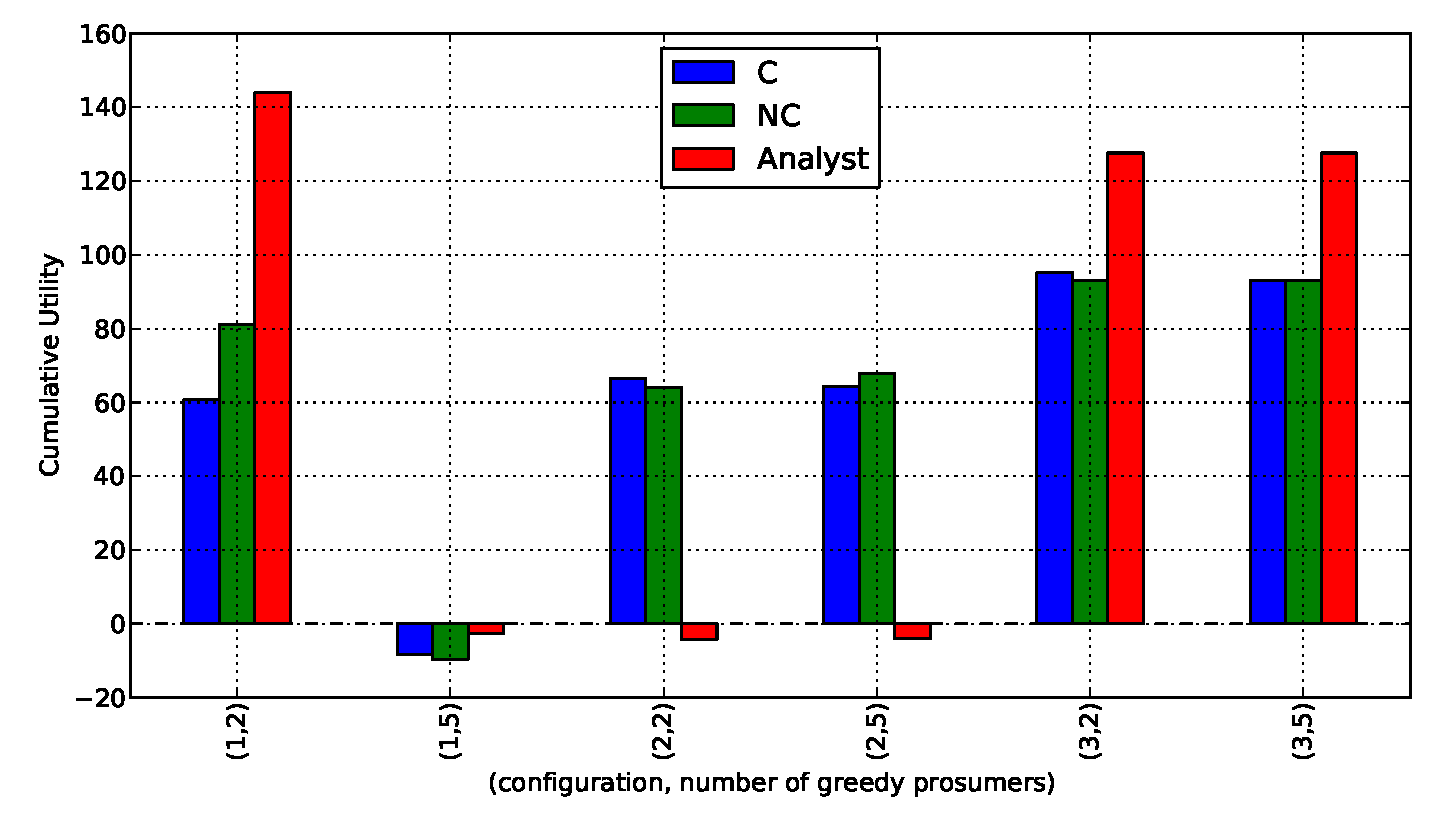
\includegraphics[width=\linewidth]{gfx/kc/measuringCost1.pdf} 
% \caption{Average cumulative utilities for Compliant prosumer (C), Non-compliant prosumer (N) and Analyst groups under three institution configurations and with 2 and 5 N agents.}\label{fig:measuringCost}
% \end{figure}

% From the graph we can see that properly compensating the analyst allows for better knowledge to be generated.

\subsection{Self-Organisation}

We have seen in the previous experiments that we firstly require several
mechanisms in place to successfully provision an enduring and efficient
institution, and secondly the optimal configuration of this institution
depends on several factors, including the cost of measuring rewards, the cost
of facilities, and the greediness of the agents using the institution.
In real-world scenarios these factors are unlikely to be static, thus a 
pre-selected equilibrium may become sub-optimal over time. Therefore we require
that these parameters can be adjusted over time, and can use the institution's
voting mechanism to do so.

We test three different approaches to self-organisation of the institution.
Firstly, centralisation\footnote{As the organisation of the system originates with an agent inside the system this centralisation still counts as self-organisation. Additionally, we use this paradigm mainly as a benchmark to evaluate `full' self-organisation paradigms.}
, where control is concentrated with one individual who
determines the best course of action on behalf of the other users. Secondly,
in a market situation agents act individually in their best interests, and the
balance between supply and demand should result in an optimal equilibrium.
Finally, we have a collective approach, where we apply Ostrom's third principle and enfranchise all individuals who
are affected by a rule in its modifications.

We firstly present how these self-organisational paradigms are implemented
with our institution specification. We then provide an initial benchmark of
these approaches, under the same scenarios as in the previous round of
experiments. This provides an initial evaluation of the relative benefits of
these paradigms under different conditions. We then perform a series of
experiments to test the power of individuals under each paradigm. This power
is measured as the extent to which agents can benefit themselves by switching
to a greedy profile. This provides a measure of the system's robustness to
manipulation by self-interested parties, and exploitation of certain groups of
agents.

\subsubsection*{Institutional Configurations}

We can implement all three of these paradigms through correct configuration of the institution. 

A centralised institution is created as follows:

\begin{itemize}
\item Facility costs paid via a subscription charged to \emph{consumers} and \emph{analysts}.
\item Fees are used to incentivise provision of artifacts as before.
\item Subscription and appropriation fees are set by the \emph{initiator} only.
\end{itemize}

Agents can create a market as follows:

\begin{itemize}
\item Each \texttt{PlayerAgent} has their own institution with a \texttt{Measured} pool. They are the sole agent occupying the \emph{gatherer} role, and thus the only one able to provision to this pool.
\item Each \emph{analyst} agent has their own institution with a \texttt{Prediction} pool. They are the sole agent occupying the \emph{analyst} role.
\item Each \texttt{PlayerAgent} occupies the role of \emph{consumer} in each of the analyst's institutions.
\item Each \emph{analyst} occupies the role of \emph{analyst} in each of the \texttt{PlayerAgent}'s institutions.
\item Each agent has individual control over the appropriation rates in their own institution.
\end{itemize}

This mimics a market as each producer has control over the price of their goods, and all consumers can choose who to purchase from.

Finally, collective governance is achieved with the same configuration as for centralised, except we enfranchise all agents who pay or receive a fee in the vote over its value, in order to satisfy Ostrom's Principle 3. Thus we have the following:

\begin{itemize}
\item \emph{consumers} and \emph{analysts} may vote on subscription fees,
\item \emph{gatherers} and \emph{analysts} may vote on the cost of \texttt{Measured} artifacts,
\item \emph{consumers} and \emph{analysts} may vote on the cost of \texttt{Predictor} artifacts.
\end{itemize}

\begin{table}
\centering
\caption{Vote enfranchisement in centralised, market and collective systems.}\label{tab:enfranchisement}
\begin{tabularx}{\textwidth}{c|lll}
Role & \multicolumn{1}{c}{Centralised} & \multicolumn{1}{c}{Market} & \multicolumn{1}{c}{Collective} \\
\hline
\multirow{3}{*}{\emph{initiator}} & subscription fee & \multirow{3}{*}{--} & \multirow{3}{*}{subscription fee} \\
& measured cost & & \\
& prediction cost & & \\
\hline
\multirow{3}{*}{\emph{analyst}} & \multirow{3}{*}{--} &  \multirow{3}{*}{own prediction cost} & subscription fee \\
& & & measured cost \\
& & & prediction cost \\
\hline
\multirow{2}{*}{\emph{gatherer}} & \multirow{2}{*}{--} & \multirow{2}{*}{own measured cost} & subscription fee \\
& & & measured cost \\
\hline
\multirow{2}{*}{\emph{consumer}} & \multirow{2}{*}{--} & \multirow{2}{*}{--} & subscription fee \\
& & & prediction cost \\
\end{tabularx}
\end{table}

Note that as populations in each role are uneven, we weight votes in order
that each group has equal voting power. For example, when there is one analyst
agent, the weight of his vote is increased such that it is equal to that of all
of the prosumers combined. This prevents his choice being drowned out by the
majority role.

We tabulate the enfranchisement we have described in
\autoref{tab:enfranchisement}. This shows which of the three issues
(subscription fees, measured cost and prediction costs) each role is empowered
to vote on. Note that in a market it is only within their own personal pool
that agents can set costs.

In each of these scenarios votes may be called periodically by an empowered
agent. For these simulations we compel these agents to do so regularly, such
that he cannot prevent a change by simply not calling any votes. We do this
with a rule which creates an obligation to open a ballot every ten time-steps.
This is accompanied by a  rule which ensures that the ballot is also closed in
a timely manner. These rules are shown in \autoref{lst:periodicballot}.

In all votes we determine winners using a Borda-count protocol. 

\begin{drools}[label=lst:periodicballot,caption=Rules to force opening and closing of ballots]
rule "Force periodic vote"
	when
		T(t % 10 == 1)
		$issue : Issue($cfv : cfvRoles, $i : inst)
		RoleOf($a : actor, inst == $i, $cfv contains role)
	then
		OpenBallot act = new OpenBallot($a, $i, $issue);
		insert( new Obl($a, act) );
end
rule "Close opened ballot"
	when
		T($t : t)
		OpenBallot(t < $t, $issue : issue, $i : inst, $a : actor)
		$b : Ballot( issue == $issue, status == Ballot.Status.OPEN )
	then
		CloseBallot act = new CloseBallot($a, $i, $b);
		insert( new Obl($a, act) );
end//$
\end{drools}

% We have seen in the previous section that we require several mechanisms in place to create an effective institution. Using static examples allows us to test certain situations, however for long-term robustness we require that these fluents, such as subscription fees, and provision and appropriate fees, can be changed over time to react to external and internal conditions. We also require that the agents in the system can do this themselves, without external supervision, so that the system is self-organised.

% We do this by allowing these fluents to be changed by vote. Periodically agents are permitted to vote on the value of a fluent, and if the vote is decisive, the value is changed. With this method we can define three models of institutional governance:
% \begin{itemize}
% \item Centralised --- A single agent has the power to vote on all issues.
% \item Market --- Those who provision an artifact (\ie supply) have the power to vote on its price.
% \item Principled --- Following Ostrom's third principle, those affected by an operational rule are permitted to vote on it: Anyone with provision or appropriation rights to a pool can vote on its fees.
% \end{itemize}

\subsubsection*{Comparison of paradigms}

We start by testing these paradigms under the same four scenarios as in the
previous experiments (described in \autoref{tab:scenarios}). This is to test
that the organisational configuration is capable of finding an appropriate
equilibrium under these static conditions.

\begin{table}
\centering
\caption[Evaluation of paradigms across simulation scenarios.]{Evaluation of paradigms across simulation scenarios.}\label{tab:selforg}
\begin{tabular}{rl|rcrrr|r}
\multicolumn{1}{c}{Scen.} & Paradigm & \multicolumn{1}{c}{Rewards} & \multicolumn{1}{c}{Endures?} & \multicolumn{1}{c}{Partic.} & \multicolumn{1}{c}{Eff.} & Equity & \multicolumn{1}{c}{Total} \\
\hline \hline
1 & central & 1280 & Yes. & 100.0\% & 68.2\% & 0.88 & 1.000 \\
1 & collective & 1278 & Yes. & 100.0\% & 68.2\% & 0.86 & 0.995 \\
1 & market & 1247 & Yes. & 100.0\% & 67.6\% & 0.83 & 0.979 \\
\hline
2 & central & 1082 & Yes. & 100.0\% & 64.4\% & 0.85 & 0.999 \\
2 & collective & 972 & Yes. & 100.0\% & 62.4\% & 0.85 & 0.975 \\
2 & market & 943 & Yes. & 100.0\% & 61.2\% & 0.75 & 0.93 \\
\hline
3 & central & 1076 & Yes. & 100.0\% & 64.2\% & 0.85 & 1.000 \\
3 & collective & 839 & Yes. & 100.0\% & 58.3\% & 0.74 & 0.912 \\
3 & market & -231 & No. & 0.0\% & 0.0\% & 0.0 & -0.054 \\
\hline
4 & central & 1070 & Yes. & 100.0\% & 64.2\% & 0.86 & 1.000 \\
4 & collective & 989 & Yes. & 100.0\% & 62.9\% & 0.82 & 0.971 \\
4 & market & 967 & Yes. & 100.0\% & 62.0\% & 0.2 & 0.785 \\
\end{tabular}
\end{table}

From the results, in \autoref{tab:selforg}, we see that centralised control
performs the best in all four scenarios. This is as expected, as under this
paradigm the \emph{initiator} sets fees in the best interests of the institution,
which in this case leads to an optimal outcome. The collective voting paradigm
performs close to the centralised one, being slightly less efficient in the more
resource constrained scenarios. Finally, the market approach performs equally
well in the first two scenarios. However, in scenario 3, with high fixed costs
for utilities, it fails to endure. Additionally, in scenario 4, with three
greedy agents, overall rewards accrued are close to that of the others,
but equity is significantly reduced.

The failure of the market in scenario 3 is expected. As each individual has
their own facility in a market, having high fixed costs incurs an impossibly
high cost on the individuals. In the other two paradigms these costs are
shared.

The low equity in the market in the final scenario can be attributed to the
greedy agents exploiting being able to set higher fees or free riding.
In the first case they gain more rewards at the expense of the analyst, and
the latter the quality of predictions will be reduced for all.

% With centralised governance the initiator agent has control over subscription, gatherer pay, and analyst pay rates. Figure~\ref{fig:centralised1} shows a combination of:
% \begin{itemize}
% \item Setting subscription rates to cover facility costs.
% \item Setting a fair appropriation fee to compensate analysts.
% \item Setting a reward for provisions when there is a measuring costs to incentivise provisions.
% \end{itemize}

% \begin{figure}
% 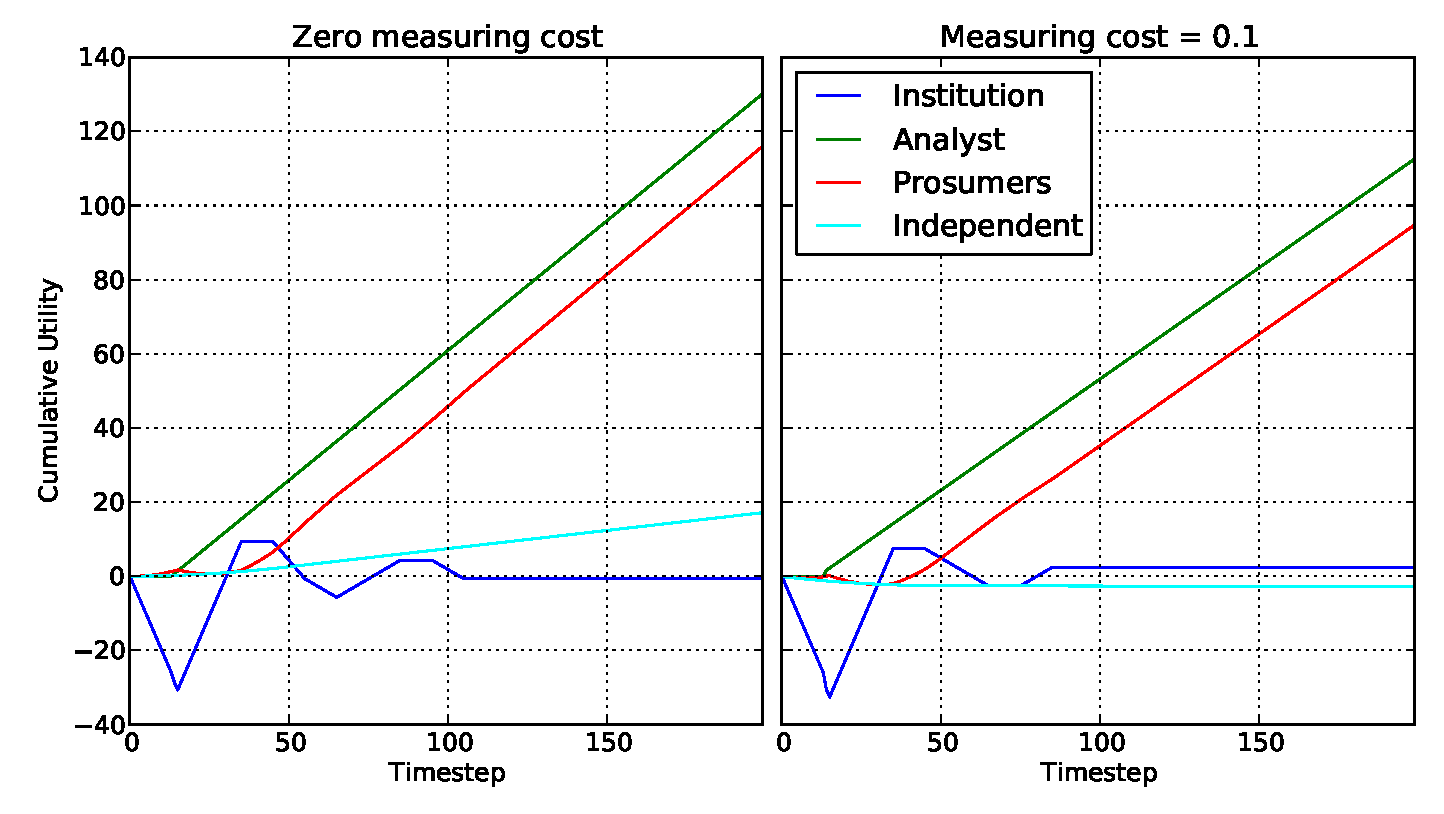
\includegraphics[width=\linewidth]{gfx/kc/centralised1.pdf} 
% \caption{Cumulative utility of agent groups over time with centralised governance, and zero and 0.1 measuring cost. Facility profile is high fixed.}\label{fig:centralised1}
% \end{figure}

% \subsubsection{Market}

% To model a basic market scenario we allow artifact suppliers to vote on the appropriation fee for their wares. Facility costs are shared by all agents.

% Figure~\ref{fig:market1} shows that the market is less efficient and robust than centralised governance. This is largely due to difficulties in the early stages of the simulation. Both analysts and prosumers are struggling to make a profit, and so raise their prices. This, in turn, means that analysts cannot afford to appropriate all available information, leading to worse knowledge for the prosumers. This effect is even more pronounced when the introduction of measuring costs further increase the scarcity of utility at the start of the simulation.

% \begin{figure}
% 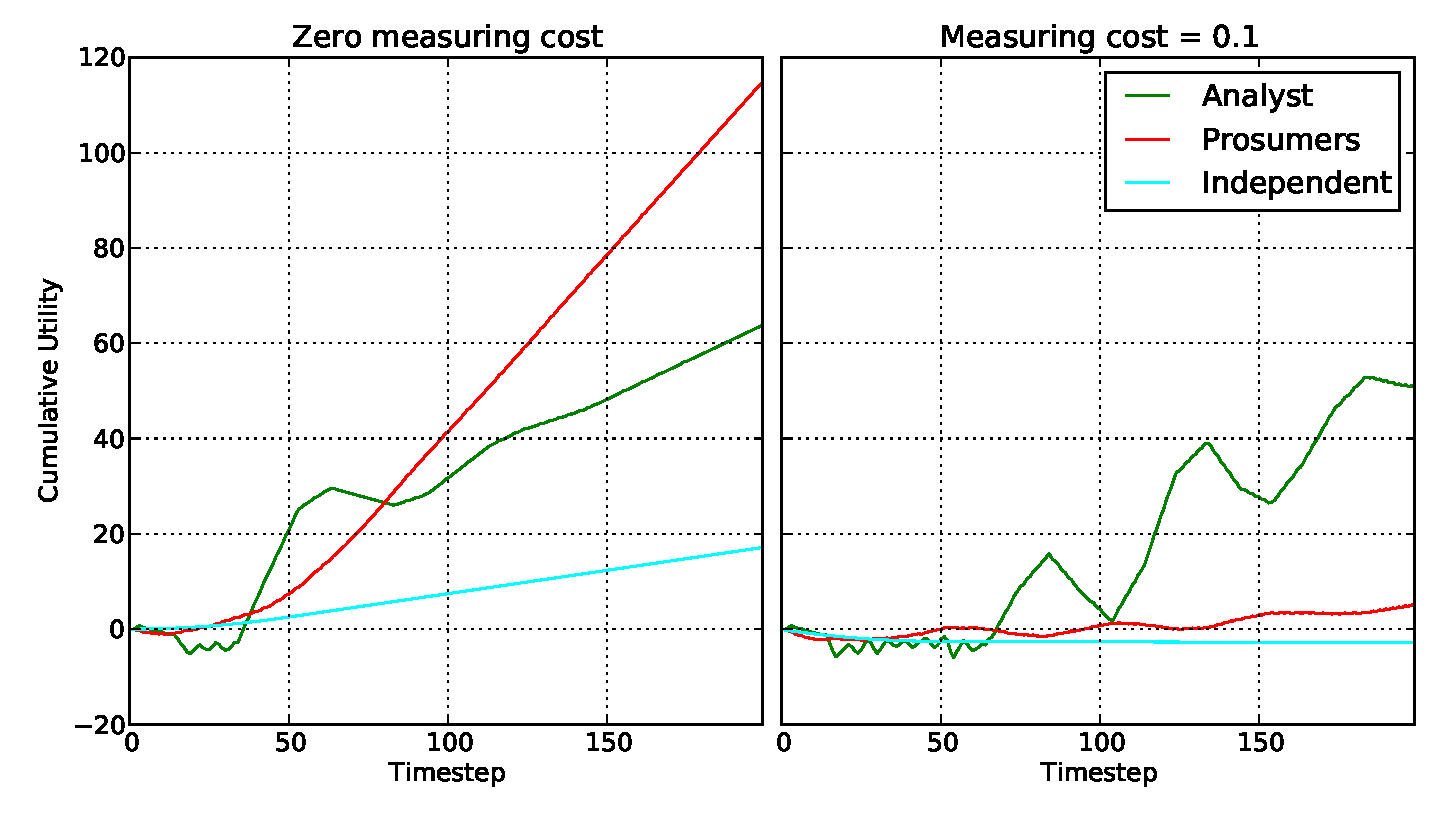
\includegraphics[width=\linewidth]{gfx/kc/market1.pdf} 
% \caption{Cumulative utility of agent groups over time with a market, and zero and 0.1 measuring cost. Facility profile is high fixed.}\label{fig:market1}
% \end{figure}

% \subsubsection{Principled}

% Under this governance scheme both analysts and prosumers can vote on appropriation rates for artifacts and a subscription fee for the institution. In order to prevent these votes being biased towards group, the ballot is weighted such that each group has an equal weighting across all its voters. Thus the vote represents a compromise across the preferences of the two groups.

% Figure~\ref{fig:principled1} shows that this governance functions comparably to centralised in compensating agents.

% \begin{figure}
% 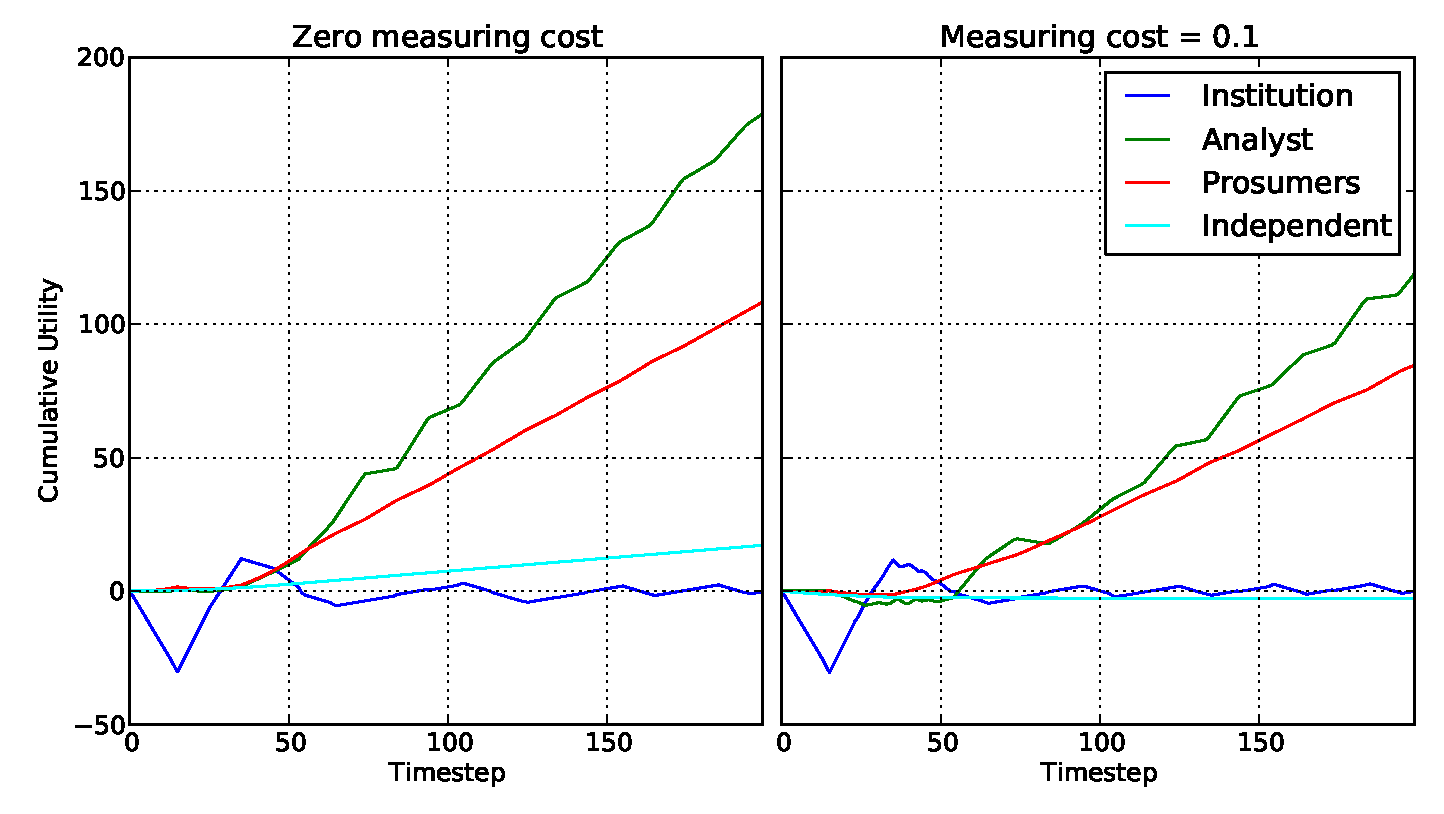
\includegraphics[width=\linewidth]{gfx/kc/principled.pdf} 
% \caption{Cumulative utility of agent groups over time with collective governance according to Ostrom's third principle, and zero and 0.1 measuring cost. Facility profile is high fixed.}\label{fig:principled1}
% \end{figure}

% \subsection{Comparison of institutional paradigms}

% We will not compare the three institutional paradigms with respect to the effect that malicious agent strategies can have on the institution.

\subsubsection*{Individual Power}

In our final experiment we test the effect of greedy actors on these
institutions, and the individual benefit which can be accrued by pursuing a
greedy strategy. If each individual can achieve a better outcome by
switching to greedy then we have a dilemma, and rational
agents will cause a tragedy of the commons through greed. 

We set up a system like Scenario 2, with flexible facility costs and a
measuring cost of $0.1$. We run this scenario with all agents in sustainable
mode in order to get a baseline measurement for each organisational paradigm.
We then test system performance with certain agents in greedy mode.
In turn, we tested each of the follow groups in greedy mode:

\begin{enumerate}
\item Agent in the role of \emph{initiator}.
\item Agent in the role of \emph{analyst}.
\item Three of the prosumer agents (\emph{gatherer} and \emph{consumer}).
\item Six of the prosumer agents.
\item All (10) of the prosumer agents
\end{enumerate}

\begin{figure}
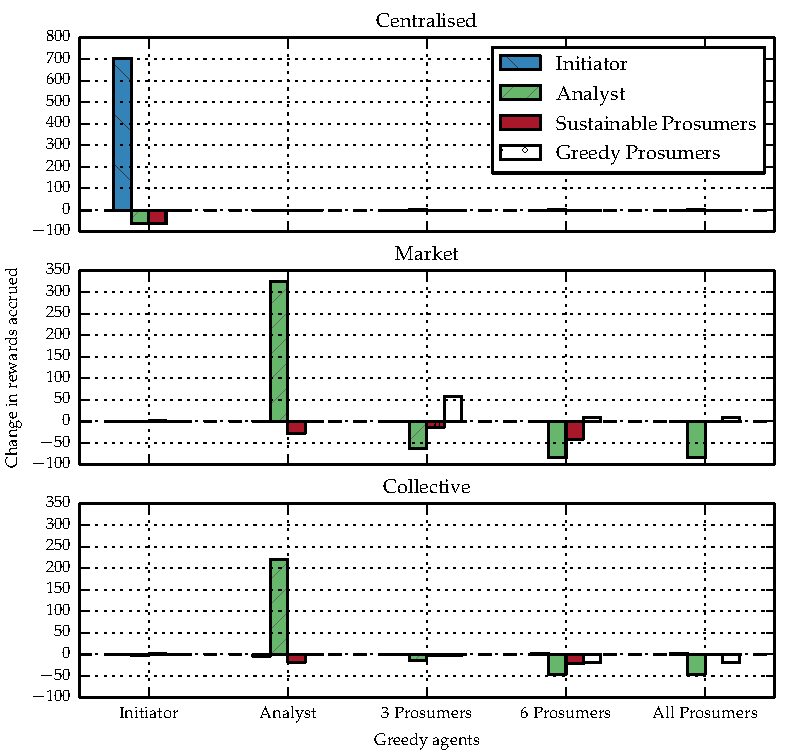
\includegraphics{gfx/kc/powerbar.pdf} 
\caption[Change in accrued rewards of agent groups with selected groups of greedy agents.]{Change in accrued rewards of agent groups with selected groups of greedy agents. Positive represents an increase in rewards over the baseline, negative a reduction.}\label{fig:powerbar}
\end{figure}

We then measure the change in utilities accrued over the simulation for each
agent type between each configuration and the baseline. With this experiment
we aim to measure the benefit to individuals, or groups of individuals, who
utilise a greedy strategy. We also test the effect on the institution, and on
its self-organisation mechanisms, of these greedy agents. The first test is a
measure of how the institutional mechanisms encourage sustainable behaviour.
The second tests the robustness of the institution to greedy behaviour, and
that a greedy minority cannot significantly negatively impact the outcomes of
well behaved agents.

\autoref{fig:powerbar} shows how individual rewards change for each group of greedy agents, when compared to the baseline.
We see that in a centralised system the \emph{initiator} is able to extract
significant benefit at the cost of the other agents, while these others have
no impact on the system at all from their non-compliance. In both of the other
systems the \emph{analyst} is able to achieve a significant improvement at a
small cost to prosumers. Greedy prosumers are also able to improve at
the cost of other agents in the market system, but this strategy fares better
when they are in the minority. When using Principle 3, there is no benefit to
greed as a prosumer.

\begin{figure}
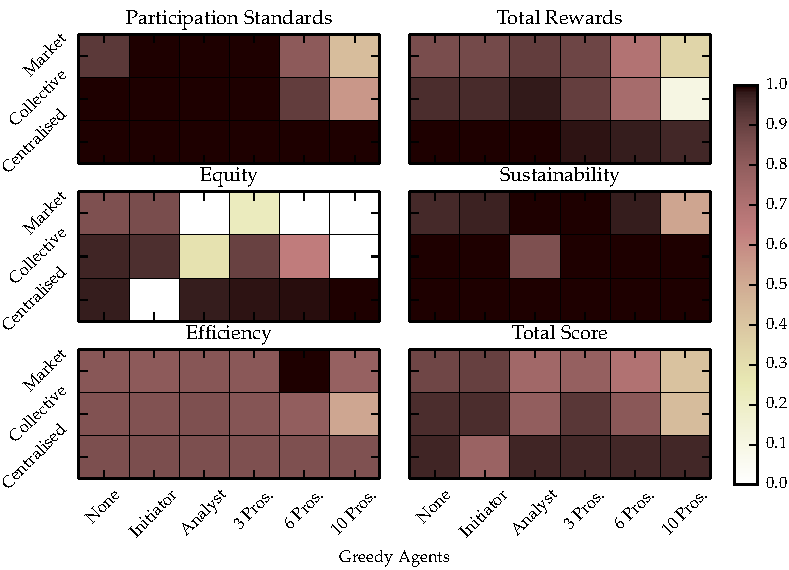
\includegraphics{gfx/kc/powercolour.pdf} 
\caption{Comparison of evaluative criteria under different organisational paradigms with different greedy agents.}\label{fig:powercolour}
\end{figure}

If we analyse these simulations further at a global level, using the
evaluative criteria we can see other effects of greed.
\autoref{fig:powercolour} shows this analysis. We can see that:

\begin{itemize}
\item The centralised solution is robust to greed, always achieving full participation and optimal rewards. However, when the \emph{initiator} is greedy, equity is lost entirely.
\item A market based solution rewards greedy behaviour, but leads to inequity when agents exploit this. High levels of greed lead to inefficiency and inequity, and therefore lower participation.
\item Using Principle 3 performs better than the market in each case. However, as the number of greedy agents approaches a majority, equity and efficiency are lost.
\end{itemize}

While the additional rewards which can be accrued by \emph{analysts} in market
and collective systems reduces the equity overall, it is worth noting
that the total system rewards in these cases is actually higher than the
baseline. The higher reward for the analyst from voting greedily allows him to
appropriate more information early in the simulation, leading better knowledge
as a result.

Additionally, when applying Principle 3, we expect that when the greedy
population approaches the majority, performance will suffer. Therefore the
fall in participation when the majority of prosumers are greedy is
expected. The voting mechanism relies on a majority working in the interests
of sustainability, and when there is none the balance is skewed towards less
optimal equilibria. This presumes that these results are rooted in the assumption
of cooperation between agents. This can generally be assumed when interactions
are repeated~\citep{Axelrod1984}.

What we see from these results is that, of the three tested organisational
paradigms, only with Principle 3 do no agents have a greed
dilemma which can lead to an unsustainable outcome, or a significantly worse
outcome for other agents. While the centralised paradigm is immune to greed by
other agents, we have demonstrated the significant power of the
\emph{initiator} to accrue significant reward for little input.

We find that the results from self-organisation are very sensitive to the
voting strategies of agents. Due to the reciprocity between roles we find that
being \emph{too} greedy often leads to the system failing to endure. Therefore,
agents must vote conservatively, with the limited information they have
available, in order to allow the agents they rely on to be able to provide for
them. This makes some exploitation by greedy agents possible, as
sustainable agents will not respond provided their accrued reward is still
within acceptable bounds.

\section{Evaluation and Conclusions}

In this chapter we have described how a subset of participatory-sensing
problems can be modelled as reinforcement-learning problems. We then described
the implementation of a simulation model which combines an abstract
reinf\-orcement-learning problem, an institution for provision and appropriation
of information and knowledge, and agents who are able to interact with the
former, using this institution in order to better exploit their combined
information and knowledge. We then showed how the evaluative criteria for the
knowledge commons, described in \autoref{sec:iad}, can generate objective
criteria from this simulation model. We presented a series of experiments
using this simulation model to show that the use of appropriate institutional
rules can be used to manage an information and knowledge commons in this
context.

These experiments represent an initial study into the value of Ostrom's
principles when applied to the knowledge commons and provision and
appropriation systems. We also demonstrate the various factors which must be
considered and accounted for in order to achieve an effective institution for
participatory sensing. This is therefore a demonstration of the problem of
supply of institutions which \citet{Ostrom1990} outlined.

The results also offer a contribution towards this problem of supply. We
demonstrate particular combinations of institutional rules and configurations
will succeed, according to the evaluative criteria. This is not an exhaustive
study of these permutations---that would be almost infeasible given the degrees of
freedom available in the configuration of the model. However, the model itself
can be a tool for institution designers to configure and test to find the
correct configuration for their domain. In this way the model is a tool for
applying Ostrom's second principle---that appropriation and provision rules
should relate to the local conditions---allowing these rules to be tested
before being deployed to a live system.

We went on to show how collective choice can be used to create a 
self-organising knowledge commons for participatory sensing. Provided agents are
able to make sufficiently intelligent voting decisions, we can shift some of
the burden of finding sustainable equilibria from the supplier of the
institution to the agents using it. By differentiating between who is
empowered to participate in collective choice we can also represent different
organisational paradigms, namely centralisation, market-based and collective
governance.

Our results with self-organisation validate our initial hypothesis from
\autoref{ch:kc}---that centralisation in participatory sensing leads to
exploitation of the data gatherers---as we showed that the \emph{initiator}
agent is able to extract significant rewards. We also showed that utilising
Ostrom's principles, specificially Principle 3 in this situation, is able to
prevent this use, and therefore that the knowledge-commons approach works in
participatory sensing.

However, this model so far only implements the first three of Ostrom's
principles. Others have been tested in isolation in other work, and
could be also investigated within our model. The implementation of the agents
and model here is such that we didn't need monitoring and sanctions in order
to sustain the system. For example, we assumed that all agents will always
perform the actions they are oliged to do. If this is not the case, then we
require principles 4, 5 and 6---monitoring, graduated sanctions and 
conflict-resolution mechanisms---to detect this non-compliance, punish it, and to
appeal when the former two are incorrectly applied. \citet{Pitt2012b}
demonstrate the use of these principles to counter such non-compliance.

From this chapter we therefore have four main contributions:
\begin{itemize}
\item A general model of participatory sensing as a reinforcement learning problem.
\item A specification and implementation of an institution for provision and appropriation of heterogeneous information and knowledge resources.
\item An experimental validation of the problem of supply in this domain, and the pitfalls in centralisation of participatory sensing.
\item An extension to the conclusion of \citet{Pitt2012b}, that Ostrom's Principles 2 and 3 lead to robustness in environmental variation, to add that they can also be used to address greed and self-interest when used in this domain.
\end{itemize}

% Inst can be seperated from the model

% \begin{itemize}
% \item The problem of supply: Institutions are hard to set-up, particularly early on.
% \item Compensating desired roles: require self-organising mechanisms to incentivise desired behaviours.
% \item Concentration of power: Too much power given to an individual can allow them to unfairly influence others' outcomes.
% \item Centralised allows the \emph{initiator} agent to extract profit at will.
% \item Market: price competition generally cancels out and also mostly prevents concentrated power. NC agents kept interested by compensation for provisions.
% \item Collective: Robust to malicious agent strategies. Requires appropriate voting rules (weighted in this case).
% \end{itemize}